% !TEX program = XeLaTeX
\documentclass[12pt,a4paper,]{article}

% Fonts
\usepackage{libertine}
% This is a nice mathfont, it fits well with Libertine
% Comment the line if you want to use a different one
\usepackage[libertine]{newtxmath}
% The default monofont 
% Again, comment the line below if you want to change it
\usepackage[scaled=.95]{inconsolata}

% Add the following packages to support kableExtra
\usepackage{booktabs}
\usepackage{longtable}
\usepackage{array}
\usepackage{multirow}
\usepackage{wrapfig}
\usepackage{colortbl}
\usepackage{pdflscape}
\usepackage{tabu}
\usepackage{threeparttable}
\usepackage{threeparttablex}
\usepackage[normalem]{ulem}
\usepackage{makecell}
\usepackage{etoolbox}
\usepackage{tocloft}
\usepackage{subcaption}


\usepackage{amsmath}
\usepackage{amssymb}
% Dots in toc
\renewcommand{\cftsecleader}{\cftdotfill{\cftdotsep}}

% Functions mignozzetti
\newcommand{\wh}[1] {\widehat { #1 }}

\newcommand{\twopd}[4]{\left\{\begin{array}{ll} #1 & \text{if } #2 \\ #3 & \text{if } #4 \end{array} \right.}

\newcommand{\twopdo}[3]{\left\{\begin{array}{ll} #1 & \text{if } #2 \\ #3 & \text{otherwise} \end{array} \right.}

\newcommand{\threepd}[6]{ \left\{ \begin{array}{lll} #1 & \text{if } #2 \\ 
#3 & \text{if } #4 \\ #5 & \text{if } #6 \end{array} \right.}

\newcommand{\threepdo}[5]{ \left\{ \begin{array}{lll} #1 & \text{if } #2 \\ 
#3 & \text{if } #4 \\ #5 & \text{otherwise} \end{array} \right.}

% Colours
\usepackage[usenames,dvipsnames]{xcolor}
\definecolor{darkblue}{rgb}{0.0,0.0,0.55}

% Spacing
\usepackage{setspace}

% Margin
\usepackage[top=2.3cm,bottom=2.3cm,left=2cm,right=2cm]{geometry}

% Packages I've been using for different reasons...
\usepackage{hyperref}
\usepackage{dcolumn}
\usepackage{graphicx}
\usepackage{float}
\floatplacement{figure}{H}
\usepackage{pgf}
\usepackage{mathtools}
\usepackage{caption}

% UK English
\usepackage[brazilian,english]{babel}
\usepackage[UKenglish]{isodate}
\cleanlookdateon

% Bold letters
\newcommand{\X}{\mathbf{X}}
\newcommand{\Y}{\mathbf{Y}}
\newcommand{\Z}{\mathbf{Z}}
\newcommand{\I}{\mathbf{I}}
\newcommand{\m}{\mathbf{m}}
\newcommand{\f}{\mathbf{f}}
\newcommand{\e}{\mathbf{e}}
\newcommand{\V}{\mathbf{V}}
\newcommand{\W}{\mathbf{W}}
\newcommand{\R}{\mathbf{R}}
\newcommand{\A}{\mathbf{A}}
\newcommand{\B}{\mathbf{B}}
\newcommand{\D}{\mathbf{D}}
\newcommand{\T}{\mathbf{T}}
\newcommand{\F}{\mathbf{F}}
\renewcommand{\O}{\mathbf{O}}
\renewcommand{\H}{\mathbf{H}}
\newcommand{\g}{\mathbf{g}}
\renewcommand{\r}{\mathbf{r}}
\newcommand{\s}{\mathbf{s}}
\newcommand{\dd}{\mathbf{d}}
\newcommand{\uu}{\mathbf{u}}
\newcommand{\w}{\mathbf{w}}
\newcommand{\x}{\mathbf{x}}
\newcommand{\vv}{\mathbf{v}}
\newcommand{\y}{\mathbf{y}}
\newcommand{\z}{\mathbf{z}}
\newcommand{\Beta}{\boldsymbol{\beta}}
\newcommand{\bveps}{\boldsymbol{\varepsilon}}
\newcommand{\bvphi}{\boldsymbol{\varphi}}
\newcommand{\btheta}{\boldsymbol{\theta}}
\newcommand{\bups}{\boldsymbol{\upsilon}}
\newcommand{\bgamma}{\boldsymbol{\gamma}}
\newcommand{\bpi}{\boldsymbol{\pi}}
\newcommand{\arrowp}{\stackrel{p}{\rightarrow}}
\newcommand{\0}{\mathbf{0}}
\newcommand{\Prob}{\mathbb{P}}
\newcommand{\E}{\mathbb{E}}
\newcommand{\nn}{\nonumber}
\newcommand{\indf}{\mathds{1}}

% Penalties
\exhyphenpenalty=1000
\hyphenpenalty=1000
\widowpenalty=1000
\clubpenalty=1000

% Hypersetup
\hypersetup{
  linkcolor=Mahogany,
  citecolor=Mahogany,
  urlcolor=darkblue, 
  breaklinks=true, 
  colorlinks=true,
      pdfauthor={João Ricardo Costa Filho},
      pdfkeywords={DSGE},
  }

% If XeTex, LuaLaTeX, etc
\usepackage{ifxetex,ifluatex}
\usepackage{fixltx2e} % provides \textsubscript
\ifnum 0\ifxetex 1\fi\ifluatex 1\fi=0 % if pdftex
  \usepackage[T1]{fontenc}
  \usepackage[utf8]{inputenc}
\else % if luatex or xelatex
  \ifxetex
    \usepackage{amssymb,amsmath}
    \usepackage{mathspec}
  \else
    \usepackage{fontspec}
  \fi
  \defaultfontfeatures{Ligatures=TeX,Scale=MatchLowercase}
\fi
% use upquote if available, for straight quotes in verbatim environments
\IfFileExists{upquote.sty}{\usepackage{upquote}}{}
% use microtype if available
\IfFileExists{microtype.sty}{%
\usepackage{microtype}
\UseMicrotypeSet[protrusion]{basicmath} % disable protrusion for tt fonts
}{}

% Language

% Bibliography
\usepackage{natbib}
\bibliographystyle{apalike}
\makeatletter
% Remove comma after author
\setcitestyle{aysep={}}
\patchcmd{\NAT@citex}
	  {\@citea\NAT@hyper@{%
		 \NAT@nmfmt{\NAT@nm}%
		 \hyper@natlinkbreak{\NAT@aysep\NAT@spacechar}{\@citeb\@extra@b@citeb}%
		 \NAT@date}}
	  {\@citea\NAT@nmfmt{\NAT@nm}%
	   \NAT@aysep\NAT@spacechar\NAT@hyper@{\NAT@date}}{}{}
	\patchcmd{\NAT@citex}
	  {\@citea\NAT@hyper@{%
		 \NAT@nmfmt{\NAT@nm}%
		 \hyper@natlinkbreak{\NAT@spacechar\NAT@@open\if*#1*\else#1\NAT@spacechar\fi}%
		   {\@citeb\@extra@b@citeb}%
		 \NAT@date}}
	  {\@citea\NAT@nmfmt{\NAT@nm}%
	   \NAT@spacechar\NAT@@open\if*#1*\else#1\NAT@spacechar\fi\NAT@hyper@{\NAT@date}}
	  {}{}
% Patch case where name and year are separated by aysep
\patchcmd{\NAT@citex}
  {\@citea\NAT@hyper@{%
     \NAT@nmfmt{\NAT@nm}%
     \hyper@natlinkbreak{\NAT@aysep\NAT@spacechar}{\@citeb\@extra@b@citeb}%
     \NAT@date}}
  {\@citea\NAT@nmfmt{\NAT@nm}%
   \NAT@aysep\NAT@spacechar\NAT@hyper@{\NAT@date}}{}{}
% Patch case where name and year are separated by opening bracket
\patchcmd{\NAT@citex}
  {\@citea\NAT@hyper@{%
     \NAT@nmfmt{\NAT@nm}%
     \hyper@natlinkbreak{\NAT@spacechar\NAT@@open\if*#1*\else#1\NAT@spacechar\fi}%
       {\@citeb\@extra@b@citeb}%
     \NAT@date}}
  {\@citea\NAT@nmfmt{\NAT@nm}%
   \NAT@spacechar\NAT@@open\if*#1*\else#1\NAT@spacechar\fi\NAT@hyper@{\NAT@date}}
  {}{}
\makeatother

% Listings
\usepackage{color}
\usepackage{fancyvrb}
\newcommand{\VerbBar}{|}
\newcommand{\VERB}{\Verb[commandchars=\\\{\}]}
\DefineVerbatimEnvironment{Highlighting}{Verbatim}{commandchars=\\\{\}}
% Add ',fontsize=\small' for more characters per line
\usepackage{framed}
\definecolor{shadecolor}{RGB}{248,248,248}
\newenvironment{Shaded}{\begin{snugshade}}{\end{snugshade}}
\newcommand{\AlertTok}[1]{\textcolor[rgb]{0.94,0.16,0.16}{#1}}
\newcommand{\AnnotationTok}[1]{\textcolor[rgb]{0.56,0.35,0.01}{\textbf{\textit{#1}}}}
\newcommand{\AttributeTok}[1]{\textcolor[rgb]{0.77,0.63,0.00}{#1}}
\newcommand{\BaseNTok}[1]{\textcolor[rgb]{0.00,0.00,0.81}{#1}}
\newcommand{\BuiltInTok}[1]{#1}
\newcommand{\CharTok}[1]{\textcolor[rgb]{0.31,0.60,0.02}{#1}}
\newcommand{\CommentTok}[1]{\textcolor[rgb]{0.56,0.35,0.01}{\textit{#1}}}
\newcommand{\CommentVarTok}[1]{\textcolor[rgb]{0.56,0.35,0.01}{\textbf{\textit{#1}}}}
\newcommand{\ConstantTok}[1]{\textcolor[rgb]{0.00,0.00,0.00}{#1}}
\newcommand{\ControlFlowTok}[1]{\textcolor[rgb]{0.13,0.29,0.53}{\textbf{#1}}}
\newcommand{\DataTypeTok}[1]{\textcolor[rgb]{0.13,0.29,0.53}{#1}}
\newcommand{\DecValTok}[1]{\textcolor[rgb]{0.00,0.00,0.81}{#1}}
\newcommand{\DocumentationTok}[1]{\textcolor[rgb]{0.56,0.35,0.01}{\textbf{\textit{#1}}}}
\newcommand{\ErrorTok}[1]{\textcolor[rgb]{0.64,0.00,0.00}{\textbf{#1}}}
\newcommand{\ExtensionTok}[1]{#1}
\newcommand{\FloatTok}[1]{\textcolor[rgb]{0.00,0.00,0.81}{#1}}
\newcommand{\FunctionTok}[1]{\textcolor[rgb]{0.00,0.00,0.00}{#1}}
\newcommand{\ImportTok}[1]{#1}
\newcommand{\InformationTok}[1]{\textcolor[rgb]{0.56,0.35,0.01}{\textbf{\textit{#1}}}}
\newcommand{\KeywordTok}[1]{\textcolor[rgb]{0.13,0.29,0.53}{\textbf{#1}}}
\newcommand{\NormalTok}[1]{#1}
\newcommand{\OperatorTok}[1]{\textcolor[rgb]{0.81,0.36,0.00}{\textbf{#1}}}
\newcommand{\OtherTok}[1]{\textcolor[rgb]{0.56,0.35,0.01}{#1}}
\newcommand{\PreprocessorTok}[1]{\textcolor[rgb]{0.56,0.35,0.01}{\textit{#1}}}
\newcommand{\RegionMarkerTok}[1]{#1}
\newcommand{\SpecialCharTok}[1]{\textcolor[rgb]{0.00,0.00,0.00}{#1}}
\newcommand{\SpecialStringTok}[1]{\textcolor[rgb]{0.31,0.60,0.02}{#1}}
\newcommand{\StringTok}[1]{\textcolor[rgb]{0.31,0.60,0.02}{#1}}
\newcommand{\VariableTok}[1]{\textcolor[rgb]{0.00,0.00,0.00}{#1}}
\newcommand{\VerbatimStringTok}[1]{\textcolor[rgb]{0.31,0.60,0.02}{#1}}
\newcommand{\WarningTok}[1]{\textcolor[rgb]{0.56,0.35,0.01}{\textbf{\textit{#1}}}}

% Verbatim

% Tables

% Graphics

% Make links footnotes instead of hotlinks:
%  \setlength{\emergencystretch}{3em}  % prevent overfull lines
 \providecommand{\tightlist}{%
   \setlength{\itemsep}{0pt}\setlength{\parskip}{0pt}}
   
% Numbered sections
\setcounter{secnumdepth}{5}
% % % Redefines (sub)paragraphs to behave more like sections
% \ifx\paragraph\undefined\else
% \let\oldparagraph\paragraph
% \renewcommand{\paragraph}[1]{\oldparagraph{#1}\mbox{}}
% \fi
% \ifx\subparagraph\undefined\else
% \let\oldsubparagraph\subparagraph
% \renewcommand{\subparagraph}[1]{\oldsubparagraph{#1}\mbox{}}
% \fi
% 
% Spacing
\doublespacing

% Title
\title{Econometria Bayesiana - Aula 11}
\providecommand{\subtitle}[1]{}
\subtitle{This is the subtitle}

% Author
\author{João Ricardo Costa Filho\footnote{Mestrado Profissional em Economia,
  Escola de Economia de São Paulo/Fundação Getúlio Vargas,
  \href{mailto:joao.costa@fgv.br}{\texttt{joao.costa@fgv.br}},
  \url{https://sites.google.com/site/joaoricardocostafilho}.}}

% Date
\date{Outubro-Dezembro, 2019}

% Begin document
\begin{document}
\maketitle

% Abstract
\begin{abstract}
\doublespacing \noindent Neste aula abordaremos a estimação bayesiana de modelos de equilíbrio
geral dinâmicas e estocásticos (DSGE no acrônimo em inglês).
\vspace{.25cm}

\noindent \textbf{Keywords}: DSGE
\vspace{.25cm}

\end{abstract}


% Table of Contents
\newpage

\hypertarget{modelos-dsge-com-estimativa-bayesiana}{%
\section{Modelos DSGE com estimativa
bayesiana}\label{modelos-dsge-com-estimativa-bayesiana}}

O exercício desta aula foi retirado de
\url{http://gecon.r-forge.r-project.org/} e replicado fielmente. Nele é
abordado um modelo da classe de RBC com governo e utilização da
capacidade instalada.

\begin{Shaded}
\begin{Highlighting}[]
\KeywordTok{library}\NormalTok{(gEcon)}
\KeywordTok{library}\NormalTok{(gEcon.estimation)}

\KeywordTok{file.copy}\NormalTok{(}\DataTypeTok{from =} \KeywordTok{file.path}\NormalTok{(}\KeywordTok{system.file}\NormalTok{(}\StringTok{"examples"}\NormalTok{, }\DataTypeTok{package =} \StringTok{"gEcon.estimation"}\NormalTok{),}
                           \StringTok{"dsge_model.gcn"}\NormalTok{), }\DataTypeTok{to =} \KeywordTok{getwd}\NormalTok{())}
\end{Highlighting}
\end{Shaded}

\begin{verbatim}
## [1] FALSE
\end{verbatim}

\begin{Shaded}
\begin{Highlighting}[]
\NormalTok{dsge_model <-}\StringTok{ }\KeywordTok{make_model}\NormalTok{(}\StringTok{"dsge_model.gcn"}\NormalTok{)}
\end{Highlighting}
\end{Shaded}

\begin{verbatim}
## (gEcon model info): model has 5 blocks: CONSUMER, FIRM, EQUILIBRIUM, GOVERNMENT, EXOG
## (gEcon model info): model is dynamic, stochastic
## (gEcon model info): model has 20 equations with 20 variables
## (gEcon model info): model has 0 calibrating equations and 0 non-free (calibrated) parameters
## (gEcon model info): after reduction the model has 12 equations with 12 variables
## (gEcon info): R code written to 'C:/Users/jcfil/Documents/2020 1 Bayesian Econometrics/Aulas/Aula 11 - Modelos DSGE/dsge_model.model.R'
## (gEcon info): LaTeX documentation written to 'C:/Users/jcfil/Documents/2020 1 Bayesian Econometrics/Aulas/Aula 11 - Modelos DSGE/dsge_model.tex' and 'C:/Users/jcfil/Documents/2020 1 Bayesian Econometrics/Aulas/Aula 11 - Modelos DSGE/dsge_model.model.tex'; created file 'C:/Users/jcfil/Documents/2020 1 Bayesian Econometrics/Aulas/Aula 11 - Modelos DSGE/dsge_model.results.tex'
## model parsed in 0.01s
## model loaded in 0.03s
\end{verbatim}

O arquivo \textbackslash{}textit\{dsge\_model.gcn\} contém o modelo:

\begin{Shaded}
\begin{Highlighting}[]
\CommentTok{# ############################################################################}
\CommentTok{# This file is a part of gEcon.estimation                                    #}
\CommentTok{#                                                                            #}
\CommentTok{# (c) Chancellery of the Prime Minister of the Republic of Poland 2012-2015  #}
\CommentTok{# (c) Grzegorz Klima, Karol Podemski 2015-2016                               #}
\CommentTok{# License terms can be found in the file 'LICENCE'                           #}
\CommentTok{#                                                                            #}
\CommentTok{# Authors: Karol Podemski                                                    #}
\CommentTok{# ############################################################################}
\CommentTok{# RBC model with variable capacity utilization and government                                                                 }
\CommentTok{# ############################################################################}


\NormalTok{options}
\NormalTok{\{}
\NormalTok{    output logfile =}\StringTok{ }\OtherTok{TRUE}\NormalTok{;}
\NormalTok{    output LaTeX =}\StringTok{ }\OtherTok{TRUE}\NormalTok{;}
\NormalTok{    verbose =}\StringTok{ }\OtherTok{TRUE}\NormalTok{;}
\NormalTok{    output R long =}\StringTok{ }\OtherTok{TRUE}\NormalTok{;}
\NormalTok{\}}

\NormalTok{tryreduce}
\NormalTok{\{}
\NormalTok{    H_d[], PI[], lambda_U[], lambda_c[], T[], P[];}
\NormalTok{\};}

\NormalTok{block CONSUMER}
\NormalTok{\{}
\NormalTok{    definitions}
\NormalTok{    \{}
\NormalTok{        u[] =}\StringTok{ }\KeywordTok{log}\NormalTok{(C[]) }\OperatorTok{+}\StringTok{ }\NormalTok{psi }\OperatorTok{*}\StringTok{ }\KeywordTok{log}\NormalTok{(}\DecValTok{1} \OperatorTok{-}\StringTok{ }\NormalTok{H[]);}
\NormalTok{    \}}
\NormalTok{    controls}
\NormalTok{    \{}
\NormalTok{        C[], H[];}
\NormalTok{    \}}
\NormalTok{    objective}
\NormalTok{    \{}
\NormalTok{        U[] =}\StringTok{ }\NormalTok{u[] }\OperatorTok{+}\StringTok{ }\NormalTok{beta }\OperatorTok{*}\StringTok{ }\NormalTok{E[][U[}\DecValTok{1}\NormalTok{]]    }\OperatorTok{:}\StringTok{ }\NormalTok{lambda_U[];}
\NormalTok{    \}}
\NormalTok{    constraints}
\NormalTok{    \{}
\NormalTok{         C[] }\OperatorTok{+}\StringTok{ }\NormalTok{T[] =}\StringTok{ }\NormalTok{W[] }\OperatorTok{*}\StringTok{ }\NormalTok{H[] }\OperatorTok{+}\StringTok{ }\NormalTok{PI[]       }\OperatorTok{:}\StringTok{ }\NormalTok{lambda_c[];}
\NormalTok{    \}}
\NormalTok{    calibration}
\NormalTok{    \{}
\NormalTok{        beta =}\StringTok{ }\FloatTok{0.99}\NormalTok{;}
\NormalTok{        psi =}\StringTok{ }\FloatTok{1.75}\NormalTok{;}
\NormalTok{    \}}
\NormalTok{\}}


\NormalTok{block FIRM}
\NormalTok{\{}
\NormalTok{    controls}
\NormalTok{    \{}
\NormalTok{        K[], H_d[], Y[], I[], PI[], CapUt[];}
\NormalTok{    \};}
\NormalTok{    objective}
\NormalTok{    \{}
\NormalTok{        SPI[] =}\StringTok{ }\NormalTok{PI[] }\OperatorTok{+}\StringTok{ }\NormalTok{E[][lambda_U[}\DecValTok{1}\NormalTok{] }\OperatorTok{*}\StringTok{ }\NormalTok{lambda_c[}\DecValTok{1}\NormalTok{] }\OperatorTok{/}\StringTok{ }\NormalTok{lambda_c[] }\OperatorTok{*}\StringTok{ }\NormalTok{SPI[}\DecValTok{1}\NormalTok{]];}
\NormalTok{    \};}
\NormalTok{    constraints}
\NormalTok{    \{}
\NormalTok{        Y[] =}\StringTok{ }\KeywordTok{exp}\NormalTok{(Z[]) }\OperatorTok{^}\StringTok{ }\NormalTok{(}\DecValTok{1} \OperatorTok{-}\StringTok{ }\NormalTok{alpha) }\OperatorTok{*}\StringTok{ }\NormalTok{(K[}\OperatorTok{-}\DecValTok{1}\NormalTok{] }\OperatorTok{*}\StringTok{ }\NormalTok{CapUt[])}\OperatorTok{^}\NormalTok{alpha }\OperatorTok{*}\StringTok{ }\NormalTok{(H_d[] )}\OperatorTok{^}\NormalTok{(}\DecValTok{1} \OperatorTok{-}\StringTok{ }\NormalTok{alpha);}
\NormalTok{        K[] =}\StringTok{ }\NormalTok{(}\DecValTok{1} \OperatorTok{-}\StringTok{ }\NormalTok{delta }\OperatorTok{*}\StringTok{ }\NormalTok{CapUt[] }\OperatorTok{^}\StringTok{ }\NormalTok{omega) }\OperatorTok{*}\StringTok{ }\NormalTok{K[}\OperatorTok{-}\DecValTok{1}\NormalTok{]  }\OperatorTok{+}\StringTok{ }\NormalTok{I[];}
\NormalTok{        PI[] =}\StringTok{ }\NormalTok{P[] }\OperatorTok{*}\StringTok{ }\NormalTok{Y[] }\OperatorTok{-}\StringTok{ }\NormalTok{H_d[] }\OperatorTok{*}\StringTok{ }\NormalTok{W[] }\OperatorTok{-}\StringTok{ }\NormalTok{I[];}
\NormalTok{    \};}
\NormalTok{    identities}
\NormalTok{    \{}
\NormalTok{        K_ut[] =}\StringTok{ }\NormalTok{CapUt[] }\OperatorTok{*}\StringTok{ }\NormalTok{K[}\OperatorTok{-}\DecValTok{1}\NormalTok{];}
\NormalTok{    \};}
\NormalTok{    calibration}
\NormalTok{    \{}
\NormalTok{        alpha =}\StringTok{ }\FloatTok{0.33}\NormalTok{;}
\NormalTok{        omega =}\StringTok{ }\FloatTok{1.45}\NormalTok{;}
\NormalTok{        delta =}\StringTok{ }\FloatTok{0.0265}\NormalTok{;}
\NormalTok{    \}}
\NormalTok{\}}


\NormalTok{block EQUILIBRIUM}
\NormalTok{\{}
\NormalTok{    identities}
\NormalTok{    \{}
\NormalTok{        P[] =}\StringTok{ }\DecValTok{1}\NormalTok{;}
\NormalTok{        H[] =}\StringTok{ }\NormalTok{H_d[];}
\NormalTok{    \};}
\NormalTok{\};}

\NormalTok{block GOVERNMENT}
\NormalTok{\{}
\NormalTok{    identities}
\NormalTok{    \{}
\NormalTok{        T[] =}\StringTok{ }\NormalTok{G[];}
\NormalTok{        G[] =}\StringTok{ }\NormalTok{phi_G }\OperatorTok{*}\StringTok{ }\NormalTok{G[}\OperatorTok{-}\DecValTok{1}\NormalTok{] }\OperatorTok{+}\StringTok{ }\NormalTok{epsilon_G[];}
\NormalTok{    \};}
\NormalTok{    shocks}
\NormalTok{    \{}
\NormalTok{        epsilon_G[];}
\NormalTok{    \};}
\NormalTok{    calibration}
\NormalTok{    \{}
\NormalTok{        phi_G =}\StringTok{ }\FloatTok{0.9}\NormalTok{;}
\NormalTok{    \};}
\NormalTok{\};}

\NormalTok{block EXOG }
\NormalTok{\{}
\NormalTok{    identities}
\NormalTok{    \{    }
\NormalTok{        Z[] =}\StringTok{ }\NormalTok{phi_Z }\OperatorTok{*}\StringTok{ }\NormalTok{Z[}\OperatorTok{-}\DecValTok{1}\NormalTok{]  }\OperatorTok{+}\StringTok{ }\NormalTok{epsilon_Z[];}
\NormalTok{    \}}
\NormalTok{    shocks}
\NormalTok{    \{           }
\NormalTok{        epsilon_Z[];}
\NormalTok{    \}}
\NormalTok{    calibration}
\NormalTok{    \{}
\NormalTok{        phi_Z =}\StringTok{ }\FloatTok{0.9}\NormalTok{;}
\NormalTok{    \}}
\NormalTok{\};}
\end{Highlighting}
\end{Shaded}

A partir dele, podemos resolver o modelo utilizando o pacote
\textit{gEcon}. A estimativa bayesiana, via MCMC, utiliza o pactoe
\textit{gEcon.estimation}.

\begin{Shaded}
\begin{Highlighting}[]
\CommentTok{# solve the model}
\NormalTok{dsge_model <-}\StringTok{ }\KeywordTok{steady_state}\NormalTok{(dsge_model)}
\end{Highlighting}
\end{Shaded}

\begin{verbatim}
## Steady state has been FOUND
\end{verbatim}

\begin{Shaded}
\begin{Highlighting}[]
\NormalTok{dsge_model <-}\StringTok{ }\KeywordTok{solve_pert}\NormalTok{(dsge_model, }\DataTypeTok{loglin =} \OtherTok{TRUE}\NormalTok{)}
\end{Highlighting}
\end{Shaded}

\begin{verbatim}
## Model has been SOLVED
\end{verbatim}

\begin{Shaded}
\begin{Highlighting}[]
\CommentTok{# set the stochastic shocks distribution parameters}
\NormalTok{dsge_model <-}\StringTok{ }\KeywordTok{set_shock_distr_par}\NormalTok{(dsge_model,}
                                  \DataTypeTok{distr_par =} \KeywordTok{list}\NormalTok{(}\StringTok{"sd( epsilon_G )"}\NormalTok{ =}\StringTok{ }\FloatTok{0.01}\NormalTok{,}
                                                   \StringTok{"sd( epsilon_Z )"}\NormalTok{ =}\StringTok{ }\FloatTok{0.01}\NormalTok{))}
\KeywordTok{shock_info}\NormalTok{(}\DataTypeTok{model =}\NormalTok{ dsge_model, }\DataTypeTok{all =} \OtherTok{TRUE}\NormalTok{)}
\end{Highlighting}
\end{Shaded}

\begin{verbatim}
## Incidence info:
## 
##       epsilon_G epsilon_Z
## Eq. 7         X         .
## Eq. 8         .         X
## 
## ---------------------------------------------------------- 
## 
## Covariance matrix of shocks: 
## 
##           epsilon_G epsilon_Z
## epsilon_G     1e-04     0e+00
## epsilon_Z     0e+00     1e-04
\end{verbatim}

A base de dados será criada a partir de simulações do modelo:

\begin{Shaded}
\begin{Highlighting}[]
\CommentTok{# ###################################################################}
\CommentTok{# 2. simulate the model to obtain data for the estimation}
\CommentTok{# choose variables of interest}
\KeywordTok{set.seed}\NormalTok{(}\DecValTok{1301}\NormalTok{)}
\NormalTok{series_length <-}\StringTok{ }\DecValTok{150}
\NormalTok{observables <-}\StringTok{ }\KeywordTok{c}\NormalTok{(}\StringTok{"Y"}\NormalTok{, }\StringTok{"G"}\NormalTok{)}
\CommentTok{# simulate random path}
\NormalTok{dsge_simulation <-}\StringTok{ }\KeywordTok{random_path}\NormalTok{(}\DataTypeTok{model =}\NormalTok{ dsge_model,}
                               \DataTypeTok{sim_length =}\NormalTok{ series_length,}
                               \DataTypeTok{variables =}\NormalTok{ observables)}
\NormalTok{model_data <-}\StringTok{ }\KeywordTok{get_simulation_results}\NormalTok{(dsge_simulation)}

\CommentTok{# create data set to be used for estimation (ts object)}
\NormalTok{estimation_data <-}\StringTok{ }\KeywordTok{ts}\NormalTok{(}\DataTypeTok{data =} \KeywordTok{t}\NormalTok{(model_data)[, observables],}
                      \DataTypeTok{start =} \KeywordTok{c}\NormalTok{(}\DecValTok{1973}\NormalTok{, }\DecValTok{1}\NormalTok{),}
                      \DataTypeTok{frequency =} \DecValTok{4}\NormalTok{, }\DataTypeTok{names =}\NormalTok{ observables)}
\CommentTok{# remove mean from the data series}
\NormalTok{mean_var <-}\StringTok{ }\KeywordTok{matrix}\NormalTok{(}\KeywordTok{apply}\NormalTok{(estimation_data, }\DecValTok{2}\NormalTok{, mean),}
                   \DataTypeTok{byrow =} \OtherTok{TRUE}\NormalTok{,}
                   \DataTypeTok{nrow =} \KeywordTok{nrow}\NormalTok{(estimation_data),}
                   \DataTypeTok{ncol =} \KeywordTok{ncol}\NormalTok{(estimation_data))}
\NormalTok{estimation_data <-}\StringTok{ }\NormalTok{estimation_data }\OperatorTok{-}\StringTok{ }\NormalTok{mean_var}
\end{Highlighting}
\end{Shaded}

Para os parâmetros estimados, é necessário declarar a prior:

\begin{Shaded}
\begin{Highlighting}[]
\CommentTok{# ###################################################################}
\CommentTok{# 3. declare prior distribution}
\NormalTok{dsge_prior <-}\StringTok{ }\KeywordTok{gecon_prior}\NormalTok{(}
  \DataTypeTok{prior_list =} \KeywordTok{list}\NormalTok{(}
    \KeywordTok{list}\NormalTok{(}\DataTypeTok{par =} \StringTok{"sd(epsilon_Z)"}\NormalTok{, }\DataTypeTok{type =} \StringTok{"inv_gamma"}\NormalTok{,}
         \DataTypeTok{mean =} \FloatTok{0.012}\NormalTok{, }\DataTypeTok{sd =} \FloatTok{0.3}\NormalTok{, }\DataTypeTok{lower_bound =} \FloatTok{0.0001}\NormalTok{,}
         \DataTypeTok{upper_bound =} \FloatTok{0.9}\NormalTok{, }\DataTypeTok{initial =} \FloatTok{0.0012}\NormalTok{),}
    \KeywordTok{list}\NormalTok{(}\DataTypeTok{par =} \StringTok{"sd(epsilon_G)"}\NormalTok{, }\DataTypeTok{type =} \StringTok{"inv_gamma"}\NormalTok{,}
         \DataTypeTok{mean =} \FloatTok{0.008}\NormalTok{, }\DataTypeTok{sd =} \FloatTok{0.3}\NormalTok{, }\DataTypeTok{lower_bound =} \FloatTok{0.0001}\NormalTok{,}
         \DataTypeTok{upper_bound =} \FloatTok{0.9}\NormalTok{, }\DataTypeTok{initial =} \FloatTok{0.006}\NormalTok{),}
    \KeywordTok{list}\NormalTok{(}\DataTypeTok{par =} \StringTok{"omega"}\NormalTok{, }\DataTypeTok{type =} \StringTok{"normal"}\NormalTok{,}\DataTypeTok{mean =} \FloatTok{1.45}\NormalTok{, }\DataTypeTok{sd =} \FloatTok{0.1}\NormalTok{, }\DataTypeTok{lower_bound =} \DecValTok{1}\NormalTok{,}
         \DataTypeTok{upper_bound =} \DecValTok{2}\NormalTok{, }\DataTypeTok{initial =} \FloatTok{1.5}\NormalTok{),}
    \KeywordTok{list}\NormalTok{(}\DataTypeTok{par =} \StringTok{"phi_G"}\NormalTok{, }\DataTypeTok{type =} \StringTok{"beta"}\NormalTok{,}
         \DataTypeTok{mean =} \FloatTok{0.88}\NormalTok{, }\DataTypeTok{sd =} \FloatTok{0.03}\NormalTok{, }\DataTypeTok{lower_bound =} \FloatTok{0.5}\NormalTok{,}
         \DataTypeTok{upper_bound =} \FloatTok{0.999}\NormalTok{, }\DataTypeTok{initial =} \FloatTok{0.95}\NormalTok{),}
    \KeywordTok{list}\NormalTok{(}\DataTypeTok{par =} \StringTok{"phi_Z"}\NormalTok{, }\DataTypeTok{type =} \StringTok{"beta"}\NormalTok{,}
         \DataTypeTok{mean =} \FloatTok{0.92}\NormalTok{, }\DataTypeTok{sd =} \FloatTok{0.03}\NormalTok{, }\DataTypeTok{lower_bound =} \FloatTok{0.5}\NormalTok{,}
         \DataTypeTok{upper_bound =} \FloatTok{0.999}\NormalTok{, }\DataTypeTok{initial =} \FloatTok{0.95}\NormalTok{)),}
  \DataTypeTok{model =}\NormalTok{ dsge_model)}
\KeywordTok{plot_prior}\NormalTok{(dsge_prior)}
\end{Highlighting}
\end{Shaded}

\begin{center}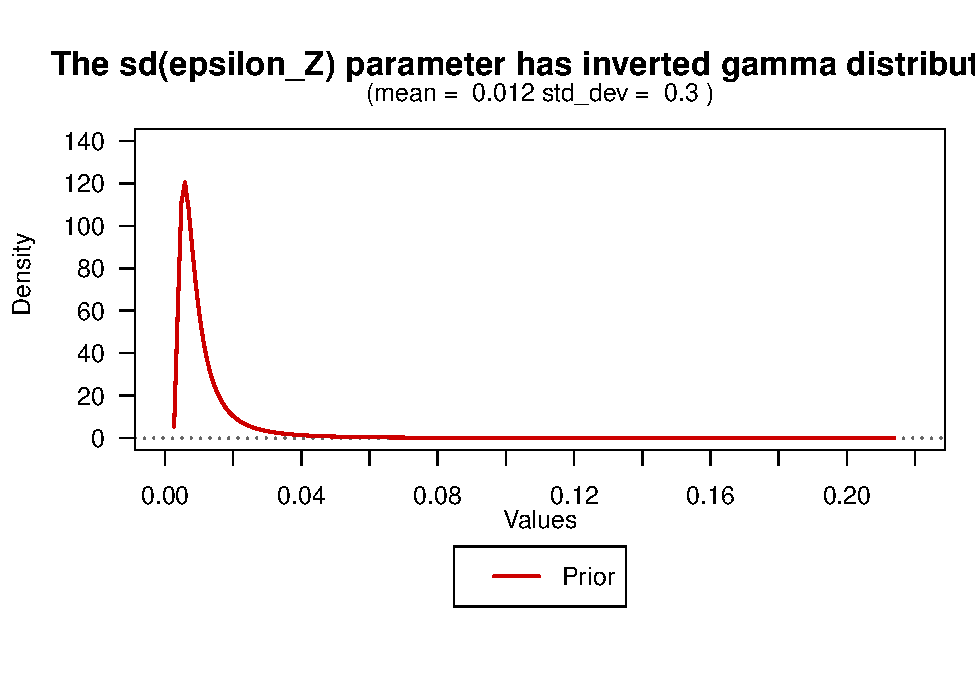
\includegraphics{figure/minimal-dsge4-1} 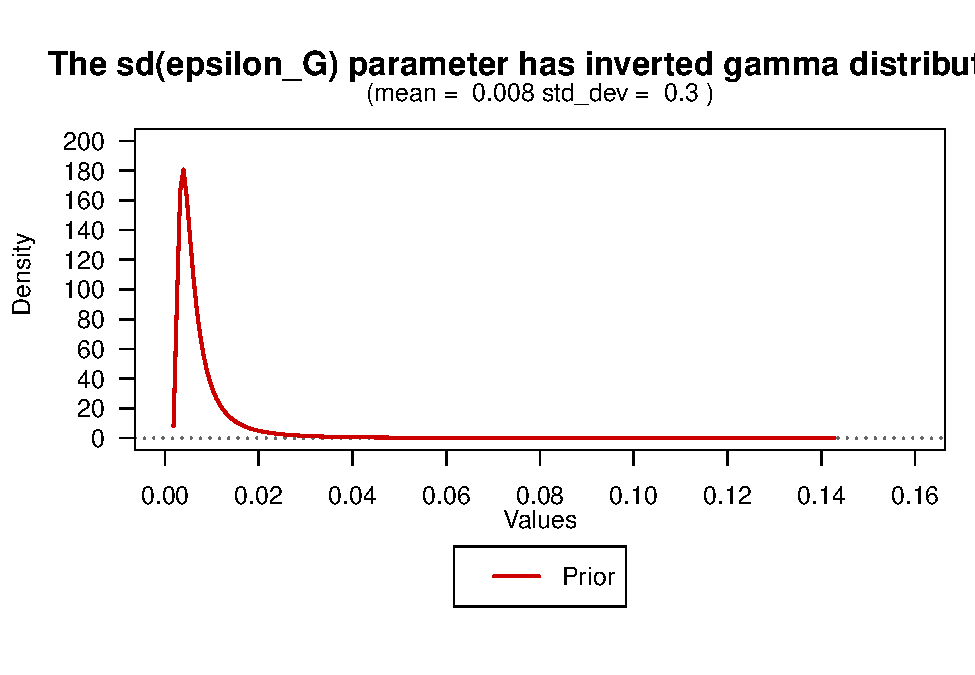
\includegraphics{figure/minimal-dsge4-2} 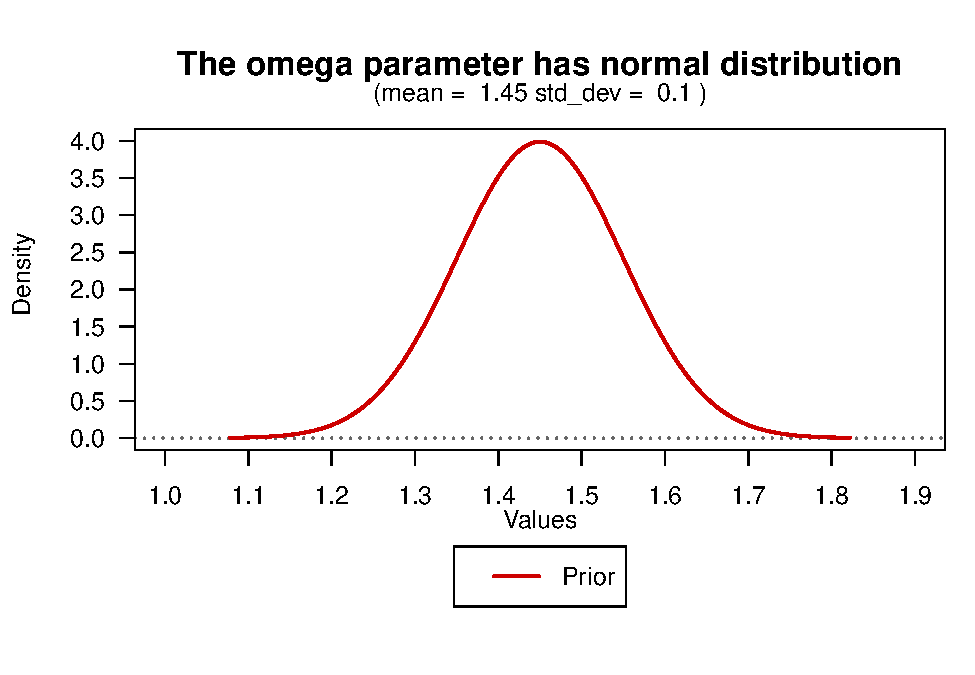
\includegraphics{figure/minimal-dsge4-3} 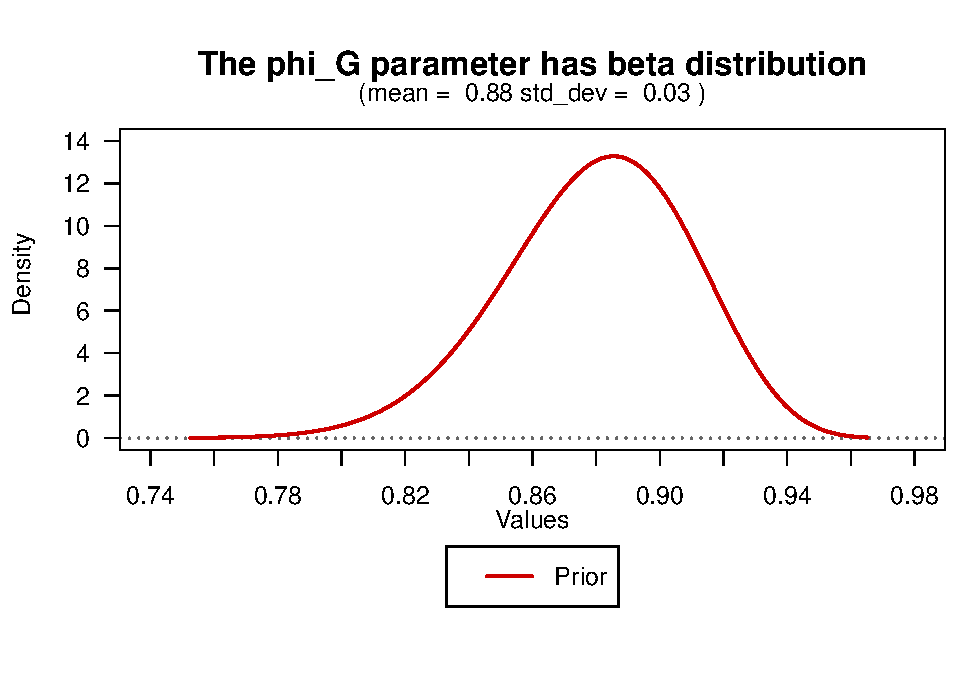
\includegraphics{figure/minimal-dsge4-4} 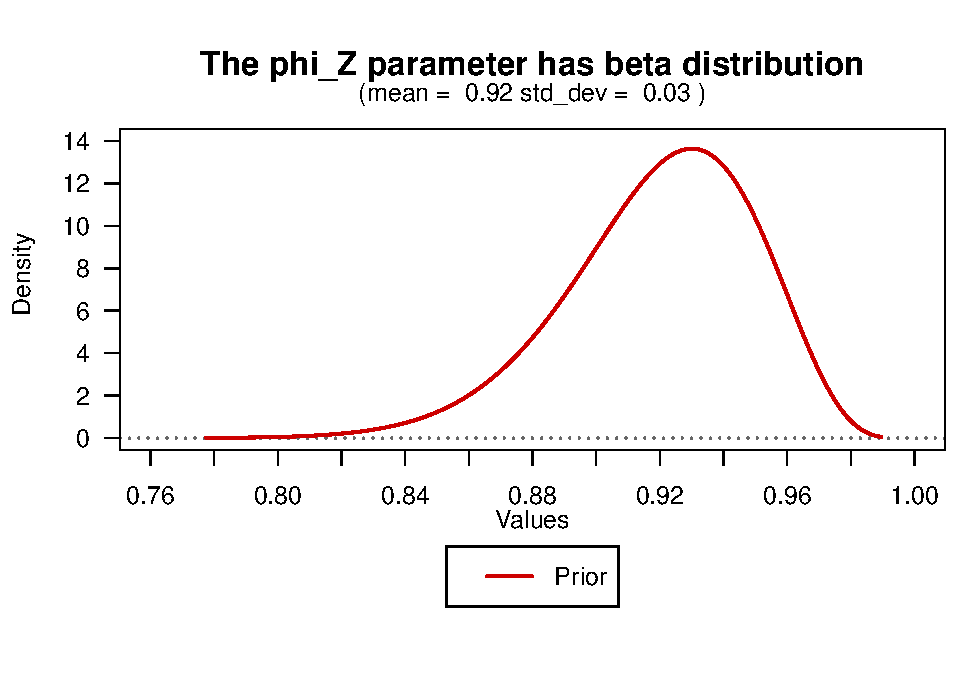
\includegraphics{figure/minimal-dsge4-5} \end{center}

\begin{Shaded}
\begin{Highlighting}[]
\CommentTok{# ###################################################################}
\CommentTok{# 4. estimate the model (Bayesian estimation)}
\NormalTok{estimation_result <-}\StringTok{ }\KeywordTok{bayesian_estimation}\NormalTok{(}\DataTypeTok{data_set =}\NormalTok{ estimation_data,}
                     \DataTypeTok{optim_options_list =} \KeywordTok{list}\NormalTok{(}\DataTypeTok{solver =} \StringTok{"csminwel"}\NormalTok{),}
                     \DataTypeTok{mcmc_options_list =} \KeywordTok{list}\NormalTok{(}\DataTypeTok{chain_length =} \DecValTok{1000}\NormalTok{,}
                     \DataTypeTok{burn =} \DecValTok{200}\NormalTok{, }\DataTypeTok{cores =} \DecValTok{2}\NormalTok{, }\DataTypeTok{chains =} \DecValTok{2}\NormalTok{, }\DataTypeTok{scale =} \KeywordTok{rep}\NormalTok{(}\FloatTok{0.5}\NormalTok{, }\DecValTok{5}\NormalTok{)),}
                     \DataTypeTok{observables =}\NormalTok{ observables, }\DataTypeTok{model =}\NormalTok{ dsge_model,}
                     \DataTypeTok{prior =}\NormalTok{ dsge_prior)}
\end{Highlighting}
\end{Shaded}

\begin{verbatim}
## 
## Finding the posterior kernel mode... 
## Moments of the distributions specified for model parameters
## 
## ---------------------------------------------------------- 
## 
## 
## Parameters of the distributions specified for model parameters
##               Distribution type 1st parameter 2nd parameter Lower bound Upper bound
## sd(epsilon_Z)         inv_gamma      2.001018  9.180268e-05       1e-04       0.900
## sd(epsilon_G)         inv_gamma      2.000453  4.076923e-05       1e-04       0.900
## omega                    normal      1.450000  1.000000e-01       1e+00       2.000
## phi_G                      beta     37.500779  1.174367e+01       5e-01       0.999
## phi_Z                      beta     30.188377  5.678290e+00       5e-01       0.999
## 
## ---------------------------------------------------------- 
## 
## 
## Initial values of parameters for estimation 
##               Initial value
## sd(epsilon_Z)        0.0012
## sd(epsilon_G)        0.0060
## omega                1.5000
## phi_G                0.9500
## phi_Z                0.9500
## 
## Initial values of the parameters:
## sd(epsilon_Z) sd(epsilon_G)         omega         phi_G         phi_Z 
##        0.0012        0.0060        1.5000        0.9500        0.9500 
## -----------------
## -----------------
## f at the beginning of new iteration,      4178.7185568636 
## x =
## sd(epsilon_Z) sd(epsilon_G)         omega         phi_G         phi_Z 
##        0.0012        0.0060        1.5000        0.9500        0.9500 
## Predicted improvement            = 3952890071.063458443
## lambda =          1; f =                  Inf 
## lambda =    0.33333; f =                  Inf 
## lambda =    0.11111; f =                  Inf 
## lambda =   0.037037; f =                  Inf 
## lambda =   0.012346; f =                  Inf 
## lambda =  0.0041152; f =                  Inf 
## lambda =  0.0013717; f =                  Inf 
## lambda = 0.00045725; f =         -393.5121068 
## lambda = 0.00015242; f =         -537.3110320 
## lambda = 5.0805e-05; f =         -685.4196998 
## Norm of dx     889.14
## ----
## Improvement on iteration        1 =     4864.138256708
## -----------------
## -----------------
## f at the beginning of new iteration,      -685.4196998443 
## x =
##    sd(epsilon_Z)    sd(epsilon_G)            omega            phi_G            phi_Z 
## 0.04637236808803 0.00622118752743 1.49999075162238 0.94998149932255 0.94983311453703 
## Predicted improvement            =    69740.486512142
## lambda =          1; f =                  Inf 
## lambda =    0.33333; f =                  Inf 
## lambda =    0.11111; f =         -235.6910904 
## lambda =   0.037037; f =         -397.3360515 
## lambda =   0.012346; f =         -549.8577104 
## lambda =  0.0041152; f =         -671.8414608 
## lambda =  0.0013717; f =         -728.2831073 
## Norm of dx     3.7347
## ----
## Improvement on iteration        2 =       42.863407499
## -----------------
## -----------------
## f at the beginning of new iteration,      -728.2831073428 
## x =
##   sd(epsilon_Z)   sd(epsilon_G)           omega           phi_G           phi_Z 
## 0.0463689423677 0.0113439928884 1.4999934934136 0.9499507919232 0.9498796189698 
## Predicted improvement            =        8.038462707
## lambda =          1; f =         -749.8583104 
## lambda =     1.9332; f =                  Inf 
## lambda =     1.3017; f =         -759.5351605 
## lambda =     1.6503; f =                  Inf 
## lambda =     1.4313; f =         -757.8016483 
## lambda =      1.559; f =                  Inf 
## lambda =     1.4811; f =                  Inf 
## lambda =     1.4071; f =         -760.3490790 
## lambda =      1.451; f =                  Inf 
## lambda =     1.4245; f =         -758.9420167 
## lambda =     1.4403; f =         -754.7739277 
## lambda =     1.4564; f =                  Inf 
## Norm of dx   0.038318
## Cliff.  Perturbing search direction. 
## Predicted improvement            =        5.939755488
## lambda =          1; f =         -744.9186091 
## lambda =     1.9332; f =                  Inf 
## lambda =     1.3017; f =         -752.8886106 
## lambda =     1.6503; f =                  Inf 
## lambda =     1.4313; f =         -756.5507177 
## lambda =      1.559; f =         -758.2688900 
## lambda =      1.698; f =                  Inf 
## lambda =     1.6131; f =         -750.2299772 
## lambda =     1.6635; f =                  Inf 
## lambda =     1.6331; f =                  Inf 
## lambda =     1.6033; f =         -754.5427655 
## lambda =     1.6211; f =                  Inf 
## Norm of dx   0.030625
## Cliff again.  Try traversing
## Predicted improvement            =    10563.999600240
## lambda =          1; f =                  Inf 
## lambda =    0.33333; f =                  Inf 
## lambda =    0.11111; f =                  Inf 
## lambda =   0.037037; f =                  Inf 
## lambda =   0.012346; f =                  Inf 
## lambda =  0.0041152; f =                  Inf 
## lambda =  0.0013717; f =         -713.7832665 
## lambda = 0.00045725; f =         -734.6939098 
## Norm of dx     145.35
## ----
## Improvement on iteration        3 =        6.410802468
## -----------------
## -----------------
## f at the beginning of new iteration,      -734.6939098113 
## x =
##   sd(epsilon_Z)   sd(epsilon_G)           omega           phi_G           phi_Z 
## 0.0463329994349 0.0105920926752 1.5071921508929 0.8838996895649 0.9513643195135 
## Predicted improvement            =        6.383925458
## lambda =          1; f =         -754.6039091 
## lambda =     1.9332; f =                  Inf 
## lambda =     1.3017; f =         -762.5670698 
## lambda =     1.6503; f =                  Inf 
## lambda =     1.4313; f =                  Inf 
## lambda =     1.3141; f =         -762.3155396 
## lambda =     1.3832; f =                  Inf 
## lambda =     1.3413; f =         -760.1919361 
## lambda =     1.3663; f =                  Inf 
## lambda =     1.3513; f =         -757.7300879 
## Norm of dx   0.035095
## Cliff.  Perturbing search direction. 
## Predicted improvement            =        2.598507791
## lambda =          1; f =         -740.7213914 
## lambda =     1.9332; f =         -748.6102565 
## lambda =     3.7372; f =                  Inf 
## lambda =     2.5164; f =         -755.2408232 
## lambda =     3.1904; f =         -758.8074716 
## lambda =     4.0448; f =                  Inf 
## lambda =      3.508; f =                  Inf 
## lambda =     3.2208; f =         -755.6552392 
## lambda =     3.3902; f =                  Inf 
## lambda =     3.2875; f =                  Inf 
## lambda =     3.2274; f =         -754.2186718 
## lambda =     3.2633; f =                  Inf 
## Norm of dx   0.016065
## Cliff again.  Try traversing
## Predicted improvement            =    10394.987299974
## lambda =          1; f =                  Inf 
## lambda =    0.33333; f =                  Inf 
## lambda =    0.11111; f =                  Inf 
## lambda =   0.037037; f =                  Inf 
## lambda =   0.012346; f =                  Inf 
## lambda =  0.0041152; f =                  Inf 
## lambda =  0.0013717; f =                  Inf 
## lambda = 0.00045725; f =         -727.6418329 
## lambda = 0.00015242; f =         -733.9570609 
## lambda = 5.0805e-05; f =         -734.6207559 
## lambda = 1.6935e-05; f =         -734.6890967 
## lambda =  5.645e-06; f =         -734.6945025 
## lambda = 1.8817e-06; f =         -734.6943523 
## Norm of dx     144.19
## ----
## Improvement on iteration        4 =        0.000592650
## -----------------
## -----------------
## f at the beginning of new iteration,      -734.6945024613 
## x =
##   sd(epsilon_Z)   sd(epsilon_G)           omega           phi_G           phi_Z 
## 0.0463224709838 0.0106120035984 1.5073969482484 0.8846851695377 0.9513088877282 
## Predicted improvement            =        6.384007617
## lambda =          1; f =         -754.5729751 
## lambda =     1.9332; f =                  Inf 
## lambda =     1.3017; f =         -762.6236440 
## lambda =     1.6503; f =                  Inf 
## lambda =     1.4313; f =                  Inf 
## lambda =     1.3141; f =         -762.4150575 
## lambda =     1.3832; f =                  Inf 
## lambda =     1.3413; f =         -760.5714313 
## lambda =     1.3663; f =                  Inf 
## lambda =     1.3513; f =         -758.5461675 
## Norm of dx   0.035103
## Cliff.  Perturbing search direction. 
## Predicted improvement            =       16.208706404
## lambda =          1; f =                  Inf 
## lambda =    0.33333; f =         -750.5294528 
## lambda =    0.64439; f =                  Inf 
## lambda =     0.4339; f =         -758.3190780 
## lambda =    0.55011; f =                  Inf 
## lambda =     0.4771; f =         -761.6421231 
## lambda =    0.51965; f =         -759.4044001 
## lambda =      0.566; f =                  Inf 
## lambda =    0.53772; f =                  Inf 
## lambda =    0.51085; f =         -761.8531039 
## lambda =     0.5268; f =                  Inf 
## lambda =    0.51717; f =         -760.4768846 
## lambda =    0.52293; f =         -756.7074549 
## lambda =    0.52875; f =                  Inf 
## Norm of dx   0.090654
## Cliff again.  Try traversing
## Predicted improvement            =  1077785.084334856
## lambda =          1; f =                  Inf 
## lambda =    0.33333; f =                  Inf 
## lambda =    0.11111; f =                  Inf 
## lambda =   0.037037; f =                  Inf 
## lambda =   0.012346; f =                  Inf 
## lambda =  0.0041152; f =                  Inf 
## lambda =  0.0013717; f =                  Inf 
## lambda = 0.00045725; f =                  Inf 
## lambda = 0.00015242; f =          647.2011010 
## lambda = 5.0805e-05; f =         -717.2078695 
## lambda = 1.6935e-05; f =         -733.5677714 
## lambda =  5.645e-06; f =         -734.6584677 
## lambda = 1.8817e-06; f =         -734.7158210 
## lambda = 6.2723e-07; f =         -734.7051588 
## lambda = 2.0908e-07; f =         -734.6984447 
## lambda = 6.9692e-08; f =         -734.6958597 
## lambda = 2.3231e-08; f =         -734.6949596 
## lambda = 7.7435e-09; f =         -734.6946554 
## lambda = 2.5812e-09; f =         -734.6945535 
## Norm of dx     1468.2
## ----
## Improvement on iteration        5 =        0.021318512
## smallest step still improving too slow
## -----------------
## -----------------
## f at the beginning of new iteration,      -734.7158209729 
## x =
##   sd(epsilon_Z)   sd(epsilon_G)           omega           phi_G           phi_Z 
## 0.0463093758460 0.0105102789254 1.5091381195917 0.8826005800318 0.9508143878485 
## Predicted improvement            =        6.157210693
## lambda =          1; f =         -754.7445388 
## lambda =     1.9332; f =                  Inf 
## lambda =     1.3017; f =         -757.9185409 
## lambda =     1.6503; f =                  Inf 
## lambda =     1.4313; f =                  Inf 
## lambda =     1.3141; f =         -749.1150042 
## Norm of dx   0.039069
## ----
## Improvement on iteration        6 =       23.202719961
## warning: possible inaccuracy in H matrix
## -----------------
## -----------------
## f at the beginning of new iteration,      -757.9185409340 
## x =
##   sd(epsilon_Z)   sd(epsilon_G)           omega           phi_G           phi_Z 
## 0.0464749939924 0.0109657137928 1.5017459333558 0.8987093633317 0.9984791525119 
## Predicted improvement            =      163.715963577
## lambda =          1; f =         -738.7346637 
## lambda =    0.33333; f =         -752.7341272 
## lambda =    0.11111; f =         -760.3939693 
## Norm of dx    0.06333
## ----
## Improvement on iteration        7 =        2.475428416
## -----------------
## -----------------
## f at the beginning of new iteration,      -760.3939693496 
## x =
##   sd(epsilon_Z)   sd(epsilon_G)           omega           phi_G           phi_Z 
## 0.0463858585288 0.0108290786241 1.5064366384089 0.8973141848375 0.9934255542139 
## Predicted improvement            =        2.537664682
## lambda =          1; f =         -763.9869053 
## Norm of dx   0.036448
## ----
## Improvement on iteration        8 =        3.592935934
## -----------------
## -----------------
## f at the beginning of new iteration,      -763.9869052837 
## x =
##    sd(epsilon_Z)    sd(epsilon_G)            omega            phi_G            phi_Z 
## 0.04579274687357 0.00975882014223 1.54227652541268 0.89081569181116 0.99390725176815 
## Predicted improvement            =        1.954824342
## lambda =          1; f =         -766.9147565 
## Norm of dx   0.046707
## ----
## Improvement on iteration        9 =        2.927851182
## -----------------
## -----------------
## f at the beginning of new iteration,      -766.9147564662 
## x =
##    sd(epsilon_Z)    sd(epsilon_G)            omega            phi_G            phi_Z 
## 0.04480288334342 0.00911257475667 1.58830832338066 0.89857828050576 0.99490101555363 
## Predicted improvement            =        3.605662306
## lambda =          1; f =         -771.7619452 
## Norm of dx   0.091113
## ----
## Improvement on iteration       10 =        4.847188689
## -----------------
## -----------------
## f at the beginning of new iteration,      -771.7619451553 
## x =
##    sd(epsilon_Z)    sd(epsilon_G)            omega            phi_G            phi_Z 
## 0.04265517972214 0.00879982043818 1.67619012631028 0.92241872843960 0.99718363637463 
## Predicted improvement            =        2.479509212
## lambda =          1; f =         -775.3485069 
## Norm of dx   0.057987
## ----
## Improvement on iteration       11 =        3.586561750
## -----------------
## -----------------
## f at the beginning of new iteration,      -775.3485069057 
## x =
##    sd(epsilon_Z)    sd(epsilon_G)            omega            phi_G            phi_Z 
## 0.04110781963609 0.00918577310305 1.73362706010088 0.93017574399612 0.99803654075330 
## Predicted improvement            =        8.296851517
## lambda =          1; f =         -786.3794232 
## Norm of dx    0.14529
## ----
## Improvement on iteration       12 =       11.030916342
## -----------------
## -----------------
## f at the beginning of new iteration,      -786.3794232476 
## x =
##   sd(epsilon_Z)   sd(epsilon_G)           omega           phi_G           phi_Z 
## 0.0370501271853 0.0106894396989 1.8788074922440 0.9336282172397 0.9972732030374 
## Predicted improvement            =        8.575324596
## lambda =          1; f =                  Inf 
## lambda =    0.33333; f =         -791.5899760 
## Norm of dx    0.30367
## ----
## Improvement on iteration       13 =        5.210552715
## -----------------
## -----------------
## f at the beginning of new iteration,      -791.5899759623 
## x =
##   sd(epsilon_Z)   sd(epsilon_G)           omega           phi_G           phi_Z 
## 0.0343962893307 0.0110010281253 1.9799076993687 0.9293984288694 0.9973504252368 
## Predicted improvement            =       13.675801479
## lambda =          1; f =                  Inf 
## lambda =    0.33333; f =                  Inf 
## lambda =    0.11111; f =                  Inf 
## lambda =   0.037037; f =         -792.5872879 
## Norm of dx    0.52623
## ----
## Improvement on iteration       14 =        0.997311934
## -----------------
## -----------------
## f at the beginning of new iteration,      -792.5872878961 
## x =
##   sd(epsilon_Z)   sd(epsilon_G)           omega           phi_G           phi_Z 
## 0.0338809617438 0.0110354336197 1.9993743873259 0.9285998635403 0.9973466411754 
## Predicted improvement            =       17.274635349
## lambda =          1; f =                  Inf 
## lambda =    0.33333; f =                  Inf 
## lambda =    0.11111; f =                  Inf 
## lambda =   0.037037; f =                  Inf 
## lambda =   0.012346; f =                  Inf 
## lambda =  0.0041152; f =                  Inf 
## lambda =  0.0013717; f =                  Inf 
## lambda = 0.00045725; f =         -792.6030825 
## lambda = 0.00088394; f =         -792.6178158 
## lambda =  0.0017088; f =                  Inf 
## lambda =  0.0011506; f =                  Inf 
## lambda = 0.00090756; f =         -792.6186311 
## lambda =  0.0010464; f =                  Inf 
## lambda = 0.00096075; f =         -792.6204672 
## lambda =  0.0010113; f =                  Inf 
## lambda = 0.00098065; f =         -792.6211541 
## lambda = 0.00099891; f =                  Inf 
## lambda = 0.00098791; f =                  Inf 
## Norm of dx    0.63408
## Cliff.  Perturbing search direction. 
## H unused
## Predicted improvement            =        0.500000000
## lambda =          1; f =         -793.5725164 
## Norm of dx    0.34944
## ----
## Improvement on iteration       15 =        0.985228505
## -----------------
## -----------------
## f at the beginning of new iteration,      -793.5725164015 
## x =
##   sd(epsilon_Z)   sd(epsilon_G)           omega           phi_G           phi_Z 
## 0.0337201011216 0.0109122461979 1.9993723906370 0.9285963141057 0.9972961100271 
## Predicted improvement            =       50.565431220
## lambda =          1; f =                  Inf 
## lambda =    0.33333; f =                  Inf 
## lambda =    0.11111; f =                  Inf 
## lambda =   0.037037; f =                  Inf 
## lambda =   0.012346; f =                  Inf 
## lambda =  0.0041152; f =                  Inf 
## lambda =  0.0013717; f =                  Inf 
## lambda = 0.00045725; f =         -793.6187472 
## lambda = 0.00088394; f =                  Inf 
## lambda =  0.0005952; f =         -793.6326915 
## lambda =  0.0007546; f =                  Inf 
## lambda = 0.00065446; f =         -793.6386817 
## lambda = 0.00071283; f =                  Inf 
## lambda = 0.00067721; f =         -793.6409811 
## lambda = 0.00069836; f =         -793.6431188 
## lambda = 0.00072017; f =                  Inf 
## lambda = 0.00070701; f =         -793.6439924 
## lambda = 0.00071488; f =                  Inf 
## Norm of dx    0.88372
## Cliff.  Perturbing search direction. 
## Predicted improvement            =      105.704702547
## lambda =          1; f =                  Inf 
## lambda =    0.33333; f =                  Inf 
## lambda =    0.11111; f =                  Inf 
## lambda =   0.037037; f =                  Inf 
## lambda =   0.012346; f =                  Inf 
## lambda =  0.0041152; f =                  Inf 
## lambda =  0.0013717; f =                  Inf 
## lambda = 0.00045725; f =         -793.6691842 
## lambda = 0.00088394; f =                  Inf 
## lambda =  0.0005952; f =         -793.6983501 
## lambda =  0.0007546; f =                  Inf 
## lambda = 0.00065446; f =         -793.7108803 
## lambda = 0.00071283; f =                  Inf 
## lambda = 0.00067721; f =                  Inf 
## lambda =  0.0006567; f =         -793.7113539 
## lambda = 0.00066893; f =         -793.7139398 
## lambda = 0.00068139; f =                  Inf 
## lambda = 0.00067389; f =                  Inf 
## Norm of dx    0.93742
## Cliff again.  Try traversing
## Predicted improvement            =  3206327.141996205
## lambda =          1; f =                  Inf 
## lambda =    0.33333; f =                  Inf 
## lambda =    0.11111; f =                  Inf 
## lambda =   0.037037; f =                  Inf 
## lambda =   0.012346; f =                  Inf 
## lambda =  0.0041152; f =                  Inf 
## lambda =  0.0013717; f =                  Inf 
## lambda = 0.00045725; f =                  Inf 
## lambda = 0.00015242; f =                  Inf 
## lambda = 5.0805e-05; f =                  Inf 
## lambda = 1.6935e-05; f =                  Inf 
## lambda =  5.645e-06; f =                  Inf 
## lambda = 1.8817e-06; f =         -811.5725569 
## lambda = 3.6376e-06; f =         -829.0600205 
## lambda = 7.0322e-06; f =                  Inf 
## lambda = 4.7351e-06; f =                  Inf 
## lambda = 3.7348e-06; f =         -830.0321231 
## lambda = 4.3063e-06; f =                  Inf 
## lambda = 3.9537e-06; f =         -832.2170763 
## lambda = 4.1616e-06; f =                  Inf 
## lambda = 4.0356e-06; f =         -833.0325084 
## lambda = 4.1107e-06; f =                  Inf 
## lambda = 4.0655e-06; f =         -833.3298251 
## Norm of dx     2532.3
## ----
## Improvement on iteration       16 =       39.757308688
## back and forth on step length never finished
## -----------------
## -----------------
## f at the beginning of new iteration,      -833.3298250899 
## x =
##   sd(epsilon_Z)   sd(epsilon_G)           omega           phi_G           phi_Z 
## 0.0238567123731 0.0104361484073 1.9999943606886 0.9257570328831 0.9974632558779 
## H unused
## Predicted improvement            =        0.500000000
## lambda =          1; f =         -834.3175064 
## Norm of dx    0.47551
## ----
## Improvement on iteration       17 =        0.987681263
## -----------------
## -----------------
## f at the beginning of new iteration,      -834.3175063529 
## x =
##   sd(epsilon_Z)   sd(epsilon_G)           omega           phi_G           phi_Z 
## 0.0236745623216 0.0103634047856 1.9999921897023 0.9257537379386 0.9973815058959 
## H unused
## Predicted improvement            =        0.500000000
## lambda =          1; f =         -835.3066923 
## Norm of dx    0.58838
## ----
## Improvement on iteration       18 =        0.989185965
## -----------------
## -----------------
## f at the beginning of new iteration,      -835.3066923176 
## x =
##   sd(epsilon_Z)   sd(epsilon_G)           omega           phi_G           phi_Z 
## 0.0234836081057 0.0102953767671 1.9999899114550 0.9257502806883 0.9973024945416 
## H unused
## Predicted improvement            =        0.500000000
## lambda =          1; f =         -836.2972831 
## lambda =     1.9332; f =         -837.2051425 
## Norm of dx    0.58451
## ----
## Improvement on iteration       19 =        1.898450142
## -----------------
## -----------------
## f at the beginning of new iteration,      -837.2051424597 
## x =
##   sd(epsilon_Z)   sd(epsilon_G)           omega           phi_G           phi_Z 
## 0.0230990191197 0.0101743848317 1.9999853163083 0.9257433096164 0.9971548459491 
## H unused
## Predicted improvement            =        0.500000000
## lambda =          1; f =         -838.1981804 
## lambda =     1.9332; f =         -839.1125735 
## Norm of dx    0.57969
## ----
## Improvement on iteration       20 =        1.907431057
## -----------------
## -----------------
## f at the beginning of new iteration,      -839.1125735171 
## x =
##   sd(epsilon_Z)   sd(epsilon_G)           omega           phi_G           phi_Z 
## 0.0226886212561 0.0100770880420 1.9999803933550 0.9257358481003 0.9970165925519 
## H unused
## Predicted improvement            =        0.500000000
## lambda =          1; f =         -840.1073895 
## lambda =     1.9332; f =         -841.0265196 
## lambda =     3.7372; f =         -842.7777513 
## Norm of dx    0.59047
## ----
## Improvement on iteration       21 =        3.665177734
## -----------------
## -----------------
## f at the beginning of new iteration,      -842.7777512516 
## x =
##    sd(epsilon_Z)    sd(epsilon_G)            omega            phi_G            phi_Z 
## 0.02185792755226 0.00993473717631 1.99997036931598 0.92572067947845 0.99676572914189 
## H unused
## Predicted improvement            =        0.500000000
## lambda =          1; f =         -843.7741464 
## lambda =     1.9332; f =         -844.6973665 
## lambda =     3.7372; f =         -846.4627966 
## Norm of dx    0.61729
## ----
## Improvement on iteration       22 =        3.685045307
## -----------------
## -----------------
## f at the beginning of new iteration,      -846.4627965587 
## x =
##    sd(epsilon_Z)    sd(epsilon_G)            omega            phi_G            phi_Z 
## 0.02097872320475 0.00987420329789 1.99995957191012 0.92570441563827 0.99654020983248 
## Predicted improvement            =       59.335187752
## lambda =          1; f =         -122.6254048 
## lambda =    0.33333; f =         -871.8562435 
## Norm of dx    0.73531
## ----
## Improvement on iteration       23 =       25.393446952
## -----------------
## -----------------
## f at the beginning of new iteration,      -871.8562435107 
## x =
##    sd(epsilon_Z)    sd(epsilon_G)            omega            phi_G            phi_Z 
## 0.01511010477466 0.00817116003253 1.75501621462895 0.92135827807504 0.99187165381283 
## H unused
## Predicted improvement            =        0.500000000
## lambda =          1; f =         -872.8111603 
## Norm of dx   0.089156
## ----
## Improvement on iteration       24 =        0.954916833
## -----------------
## -----------------
## f at the beginning of new iteration,      -872.8111603440 
## x =
##    sd(epsilon_Z)    sd(epsilon_G)            omega            phi_G            phi_Z 
## 0.01507935598126 0.00828057669377 1.75501585855759 0.92135746345566 0.99186721403861 
## Predicted improvement            =        9.205190532
## lambda =          1; f =         -882.6959019 
## Norm of dx    0.20082
## ----
## Improvement on iteration       25 =        9.884741546
## -----------------
## -----------------
## f at the beginning of new iteration,      -882.6959018903 
## x =
##   sd(epsilon_Z)   sd(epsilon_G)           omega           phi_G           phi_Z 
## 0.0148862952073 0.0094482082848 1.5547108997700 0.9094825870201 0.9839219149907 
## H unused
## Predicted improvement            =        0.500000000
## lambda =          1; f =         -883.6600036 
## Norm of dx    0.20376
## ----
## Improvement on iteration       26 =        0.964101749
## -----------------
## -----------------
## f at the beginning of new iteration,      -883.6600036393 
## x =
##    sd(epsilon_Z)    sd(epsilon_G)            omega            phi_G            phi_Z 
## 0.01464616792161 0.00954110876507 1.55471057967161 0.90948075135027 0.98392718244172 
## Predicted improvement            =        7.926362770
## lambda =          1; f =         -889.1479770 
## Norm of dx   0.031204
## ----
## Improvement on iteration       27 =        5.487973373
## -----------------
## -----------------
## f at the beginning of new iteration,      -889.1479770127 
## x =
##   sd(epsilon_Z)   sd(epsilon_G)           omega           phi_G           phi_Z 
## 0.0104134378474 0.0106982062748 1.5250814741610 0.9031850881647 0.9778503464840 
## Predicted improvement            =        3.275863548
## lambda =          1; f =         -891.3684522 
## Norm of dx   0.055325
## ----
## Improvement on iteration       28 =        2.220475209
## -----------------
## -----------------
## f at the beginning of new iteration,      -891.3684522219 
## x =
##   sd(epsilon_Z)   sd(epsilon_G)           omega           phi_G           phi_Z 
## 0.0119051674017 0.0103121481403 1.4698731005164 0.9001710300962 0.9766595740125 
## Predicted improvement            =        0.751749575
## lambda =          1; f =         -892.6809610 
## Norm of dx   0.019895
## ----
## Improvement on iteration       29 =        1.312508797
## -----------------
## -----------------
## f at the beginning of new iteration,      -892.6809610184 
## x =
##   sd(epsilon_Z)   sd(epsilon_G)           omega           phi_G           phi_Z 
## 0.0112455493104 0.0103040545459 1.4506666282013 0.8968613847770 0.9727167679411 
## Predicted improvement            =        2.138741559
## lambda =          1; f =         -894.1563150 
## Norm of dx    0.05537
## ----
## Improvement on iteration       30 =        1.475353974
## -----------------
## -----------------
## f at the beginning of new iteration,      -894.1563149922 
## x =
##    sd(epsilon_Z)    sd(epsilon_G)            omega            phi_G            phi_Z 
## 0.00929476611824 0.00994596820673 1.39824565707777 0.88821650821512 0.95725086050849 
## Predicted improvement            =        0.951551073
## lambda =          1; f =         -895.1470629 
## Norm of dx  0.0024772
## ----
## Improvement on iteration       31 =        0.990747945
## -----------------
## -----------------
## f at the beginning of new iteration,      -895.1470629374 
## x =
##    sd(epsilon_Z)    sd(epsilon_G)            omega            phi_G            phi_Z 
## 0.00999738036049 0.00981089713705 1.39810983820807 0.89023014528865 0.95849646928212 
## Predicted improvement            =        0.243317905
## lambda =          1; f =         -895.5119192 
## Norm of dx   0.012746
## ----
## Improvement on iteration       32 =        0.364856262
## -----------------
## -----------------
## f at the beginning of new iteration,      -895.5119191998 
## x =
##    sd(epsilon_Z)    sd(epsilon_G)            omega            phi_G            phi_Z 
## 0.00987223335746 0.00960388529381 1.38613056881245 0.89091845084976 0.95420350499469 
## Predicted improvement            =        0.229982580
## lambda =          1; f =         -895.8404633 
## Norm of dx   0.015442
## ----
## Improvement on iteration       33 =        0.328544072
## -----------------
## -----------------
## f at the beginning of new iteration,      -895.8404632719 
## x =
##    sd(epsilon_Z)    sd(epsilon_G)            omega            phi_G            phi_Z 
## 0.00964150326575 0.00942836136127 1.37208242771161 0.89314613973793 0.94819983201983 
## Predicted improvement            =        0.230725865
## lambda =          1; f =         -896.2169310 
## Norm of dx    0.01085
## ----
## Improvement on iteration       34 =        0.376467707
## -----------------
## -----------------
## f at the beginning of new iteration,      -896.2169309793 
## x =
##    sd(epsilon_Z)    sd(epsilon_G)            omega            phi_G            phi_Z 
## 0.00941395930217 0.00935457342360 1.36394519621116 0.89579715015202 0.94153441047964 
## Predicted improvement            =        0.566148783
## lambda =          1; f =         -897.0643735 
## Norm of dx   0.015681
## ----
## Improvement on iteration       35 =        0.847442546
## -----------------
## -----------------
## f at the beginning of new iteration,      -897.0643735248 
## x =
##    sd(epsilon_Z)    sd(epsilon_G)            omega            phi_G            phi_Z 
## 0.00902379292214 0.00935961124042 1.36441898532173 0.90040879582974 0.92655975559764 
## Predicted improvement            =        0.630673562
## lambda =          1; f =         -897.9689687 
## Norm of dx   0.028269
## ----
## Improvement on iteration       36 =        0.904595132
## -----------------
## -----------------
## f at the beginning of new iteration,      -897.9689686571 
## x =
##    sd(epsilon_Z)    sd(epsilon_G)            omega            phi_G            phi_Z 
## 0.00880526933345 0.00952679912980 1.38643736156858 0.90303956944163 0.90902945186438 
## Predicted improvement            =        0.367172261
## lambda =          1; f =         -898.4254648 
## Norm of dx   0.032195
## ----
## Improvement on iteration       37 =        0.456496136
## -----------------
## -----------------
## f at the beginning of new iteration,      -898.4254647930 
## x =
##    sd(epsilon_Z)    sd(epsilon_G)            omega            phi_G            phi_Z 
## 0.00884465030593 0.00974795868987 1.41609170147484 0.90160776603376 0.89657798254267 
## Predicted improvement            =        0.041670237
## lambda =          1; f =         -898.4726186 
## Norm of dx   0.011644
## ----
## Improvement on iteration       38 =        0.047153815
## -----------------
## -----------------
## f at the beginning of new iteration,      -898.4726186084 
## x =
##    sd(epsilon_Z)    sd(epsilon_G)            omega            phi_G            phi_Z 
## 0.00885267701848 0.00983748098237 1.42682862861279 0.89941731319654 0.89264044415818 
## Predicted improvement            =        0.001613451
## lambda =          1; f =         -898.4744242 
## Norm of dx 0.00073768
## ----
## Improvement on iteration       39 =        0.001805579
## -----------------
## -----------------
## f at the beginning of new iteration,      -898.4744241874 
## x =
##    sd(epsilon_Z)    sd(epsilon_G)            omega            phi_G            phi_Z 
## 0.00886723135473 0.00985543047356 1.42712375575694 0.89874433224872 0.89258010707982 
## Predicted improvement            =        0.000119601
## lambda =          1; f =         -898.4745615 
## Norm of dx 0.00023931
## ----
## Improvement on iteration       40 =        0.000137334
## -----------------
## -----------------
## f at the beginning of new iteration,      -898.4745615212 
## x =
##    sd(epsilon_Z)    sd(epsilon_G)            omega            phi_G            phi_Z 
## 0.00886443906194 0.00985782851119 1.42711012610656 0.89852493531279 0.89267462834690 
## Predicted improvement            =        0.000020199
## lambda =          1; f =         -898.4745892 
## Norm of dx 0.00018587
## ----
## Improvement on iteration       41 =        0.000027722
## -----------------
## -----------------
## f at the beginning of new iteration,      -898.4745892432 
## x =
##    sd(epsilon_Z)    sd(epsilon_G)            omega            phi_G            phi_Z 
## 0.00886560395217 0.00985813574894 1.42701627466330 0.89848966905616 0.89283113388589 
## Predicted improvement            =        0.000004059
## lambda =          1; f =         -898.4745960 
## Norm of dx 8.8308e-05
## ----
## Improvement on iteration       42 =        0.000006712
## -----------------
## -----------------
## f at the beginning of new iteration,      -898.4745959554 
## x =
##    sd(epsilon_Z)    sd(epsilon_G)            omega            phi_G            phi_Z 
## 0.00886606256094 0.00985843043840 1.42707786085718 0.89850360423300 0.89289286638953 
## Predicted improvement            =        0.000000990
## lambda =          1; f =         -898.4745981 
## lambda =     1.9332; f =         -898.4745987 
## Norm of dx 6.8509e-05
## ----
## Improvement on iteration       43 =        0.000002706
## -----------------
## -----------------
## f at the beginning of new iteration,      -898.4745986613 
## x =
##    sd(epsilon_Z)    sd(epsilon_G)            omega            phi_G            phi_Z 
## 0.00886651900406 0.00985910431259 1.42720318699852 0.89853401924212 0.89292300140767 
## Predicted improvement            =        0.000000504
## lambda =          1; f =         -898.4745984 
## lambda =    0.33333; f =         -898.4745987 
## Norm of dx 4.7692e-05
## ih = 1 
## ----
## Improvement on iteration       44 =        0.000000026
## improvement < crit termination
## 
## The solver has stopped searching for the solution.
## 
## 
## Computes inverse Hessian of the posterior kernel at the mode: DONE.
## 
## 
## Maximisation routine solution: 
## sd(epsilon_Z) sd(epsilon_G)         omega         phi_G         phi_Z 
##   0.008866451   0.009859030   1.427188881   0.898530299   0.892917151 
## 
## Candidate for posterior mode FOUND 
## 
## Computing marginal density (Laplace approximation)
## (Log-)marginal density 
##               878.2836 
## 
## Running burn-in phase ... 
## 
## Progress:  400/2400( 17% )
## Time consumed:  00h 00m 57s
## Estimated time left:  00h 01m 27s
## Acceptance rate:  60%
## Steady state failures:  0
## Perturbation failures:  0
## 
## Burn-in phase DONE.
## 
## Running proper phase of MCMC ... 
## 
## Progress:  900/2400( 38% )
## Time consumed:  00h 01m 16s
## Estimated time left:  00h 01m 01s
## Acceptance rate:  58%
## Steady state failures:  0
## Perturbation failures:  0
## 
## Current estimates:
## 
##                 Mean       Std. dev.
## sd(epsilon_Z)   0.008931   0.0006765
## sd(epsilon_G)   0.010072   0.0005731
## omega           1.396506   0.0834375
## phi_G           0.895451   0.0165865
## phi_Z           0.894022   0.0277492
## 
## 
## Progress:  1400/2400( 58% )
## Time consumed:  00h 01m 36s
## Estimated time left:  00h 00m 41s
## Acceptance rate:  58%
## Steady state failures:  0
## Perturbation failures:  0
## 
## Current estimates:
## 
##                 Mean       Std. dev.
## sd(epsilon_Z)   0.009179   0.0007903
## sd(epsilon_G)   0.010089   0.0005727
## omega           1.427278   0.0979651
## phi_G           0.898266   0.0168379
## phi_Z           0.902131   0.0295521
## 
## 
## Progress:  1900/2400( 79% )
## Time consumed:  00h 01m 56s
## Estimated time left:  00h 00m 20s
## Acceptance rate:  58%
## Steady state failures:  0
## Perturbation failures:  0
## 
## Current estimates:
## 
##                 Mean       Std. dev.
## sd(epsilon_Z)   0.009027   0.0007940
## sd(epsilon_G)   0.010029   0.0005561
## omega           1.411469   0.1008320
## phi_G           0.897257   0.0182132
## phi_Z           0.894715   0.0308442
## 
## 
## Progress:  2400/2400( 100% )
## Time consumed:  00h 02m 16s
## Estimated time left:  00h 00m 00s
## Acceptance rate:  59%
## Steady state failures:  0
## Perturbation failures:  0
## 
## Current estimates:
## 
##                 Mean       Std. dev.
## sd(epsilon_Z)   0.008962   0.0007563
## sd(epsilon_G)   0.009977   0.0005647
## omega           1.410502   0.0970033
## phi_G           0.897292   0.0182773
## phi_Z           0.892733   0.0310480
## 
## 
## Estimation is DONE. Total time elapsed:  00h 02m 16s
\end{verbatim}

\begin{Shaded}
\begin{Highlighting}[]
\KeywordTok{plot_posterior}\NormalTok{(estimation_result)}


\CommentTok{# csminwel: http://sims.princeton.edu/yftp/optimize/}

\CommentTok{# retrieve estimates}
\CommentTok{# true model parameters were:}
\CommentTok{# sd(epsilon_Z) 0.01}
\CommentTok{# sd(epsilon_G) 0.01}
\CommentTok{# omega 1.45}
\CommentTok{# phi_G 0.9}
\CommentTok{# phi_Z 0.9}
\NormalTok{est_par <-}\StringTok{ }\KeywordTok{get_estimated_par}\NormalTok{(estimation_result)}
\end{Highlighting}
\end{Shaded}

\begin{verbatim}
## Estimated parameter values:
##                   Values:
## sd(epsilon_Z) 0.009006809
## sd(epsilon_G) 0.009898204
## omega         1.412736976
## phi_G         0.897513530
## phi_Z         0.892903359
\end{verbatim}

\begin{Shaded}
\begin{Highlighting}[]
\NormalTok{free_par <-}\StringTok{ }\NormalTok{est_par}\OperatorTok{$}\NormalTok{free_par}
\NormalTok{shock_distr_par <-}\StringTok{ }\NormalTok{est_par}\OperatorTok{$}\NormalTok{shock_distr_par}
\NormalTok{estimated_dsge_model <-}\StringTok{ }\KeywordTok{set_free_par}\NormalTok{(dsge_model, }\DataTypeTok{free_par =}\NormalTok{ free_par)}
\NormalTok{estimated_dsge_model <-}\StringTok{ }\KeywordTok{set_shock_distr_par}\NormalTok{(estimated_dsge_model, }\DataTypeTok{distr_par =}\NormalTok{ shock_distr_par)}
\NormalTok{estimated_dsge_model <-}\StringTok{ }\KeywordTok{steady_state}\NormalTok{(estimated_dsge_model)}
\end{Highlighting}
\end{Shaded}

\begin{verbatim}
## Steady state has been FOUND
\end{verbatim}

\begin{Shaded}
\begin{Highlighting}[]
\NormalTok{estimated_dsge_model <-}\StringTok{ }\KeywordTok{solve_pert}\NormalTok{(estimated_dsge_model, }\DataTypeTok{loglin =} \OtherTok{TRUE}\NormalTok{)}
\end{Highlighting}
\end{Shaded}

\begin{verbatim}
## Model has been SOLVED
\end{verbatim}

\begin{center}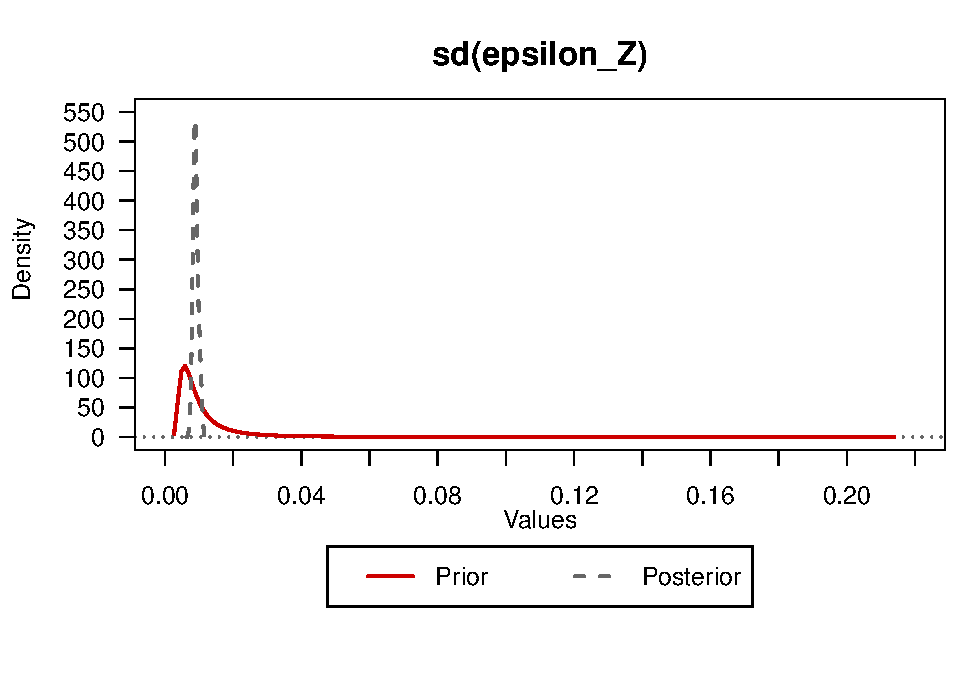
\includegraphics{figure/minimal-dsge5-1} 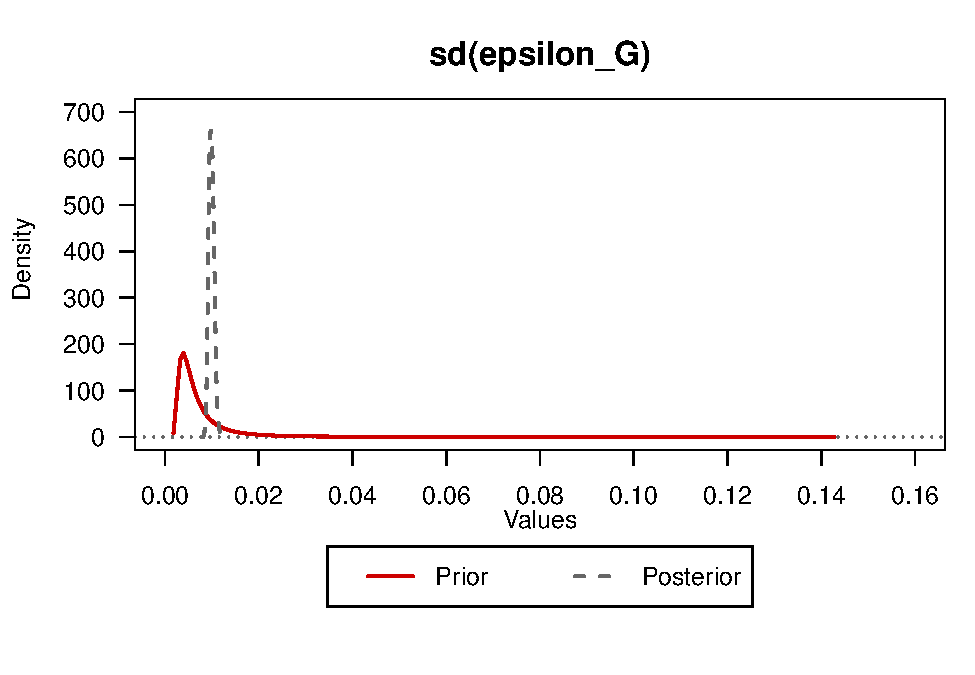
\includegraphics{figure/minimal-dsge5-2} 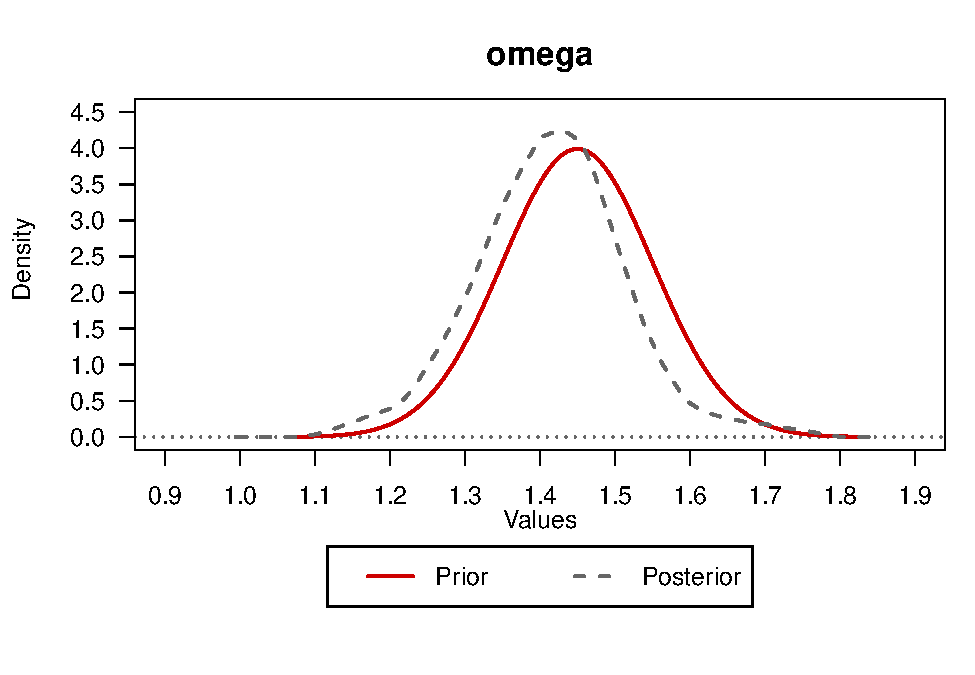
\includegraphics{figure/minimal-dsge5-3} 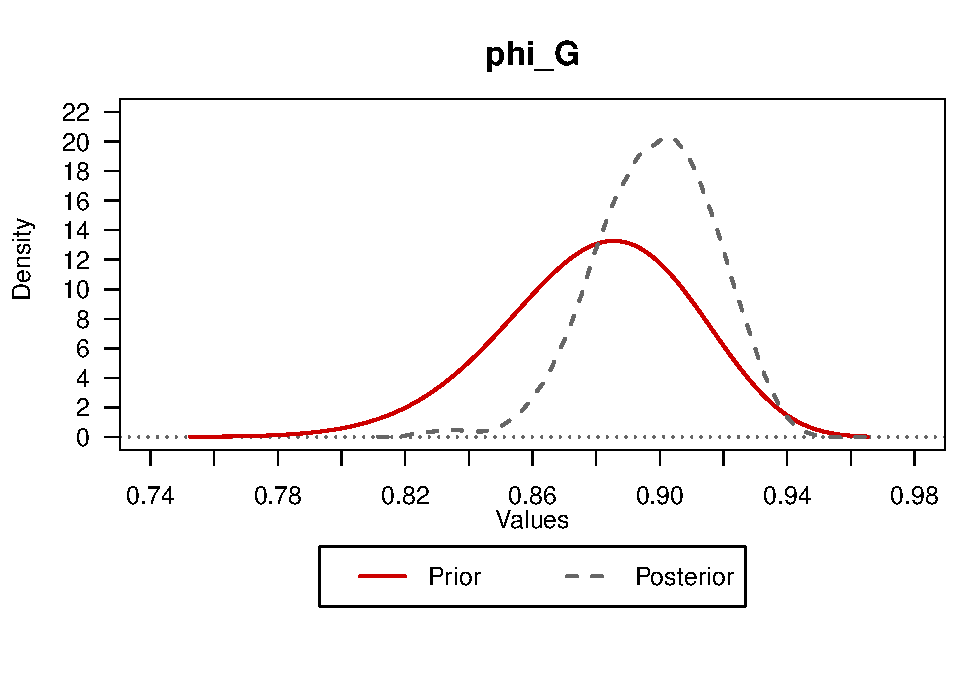
\includegraphics{figure/minimal-dsge5-4} 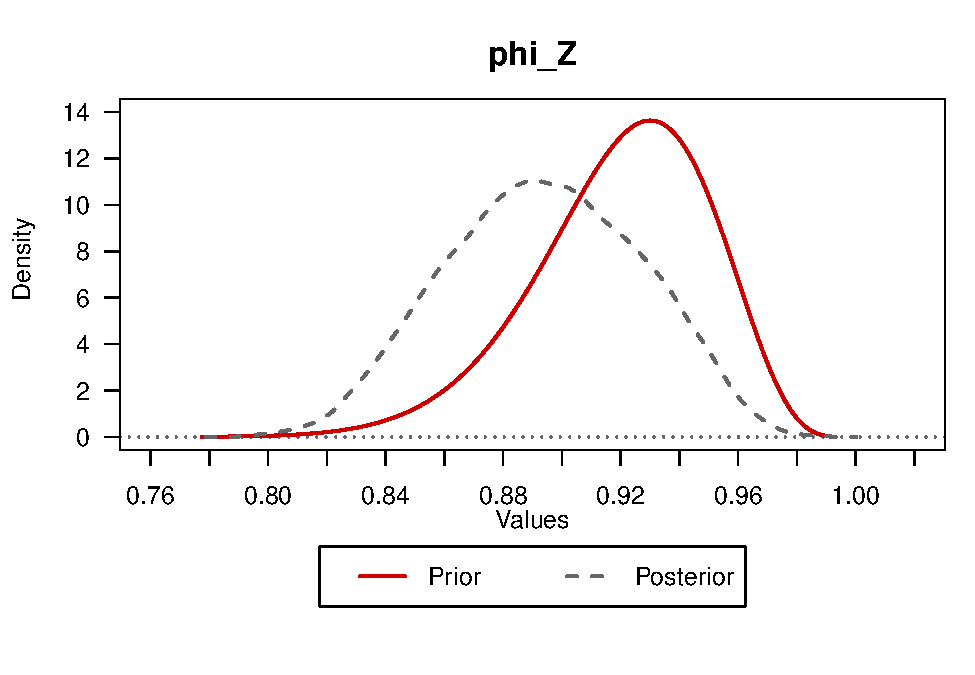
\includegraphics{figure/minimal-dsge5-5} \end{center}

\begin{Shaded}
\begin{Highlighting}[]
\CommentTok{# ###################################################################}
\CommentTok{# 5. historical shock decomposition and variable smoothing}
\CommentTok{# find historical shock decomposition}
\NormalTok{dsge_shock_decomp <-}\StringTok{ }\KeywordTok{shock_decomposition}\NormalTok{(}\DataTypeTok{model =}\NormalTok{ estimated_dsge_model,}
                                         \DataTypeTok{data_set =} \KeywordTok{window}\NormalTok{(estimation_data,}
                                                           \DataTypeTok{start =} \KeywordTok{c}\NormalTok{(}\DecValTok{2004}\NormalTok{, }\DecValTok{1}\NormalTok{),}
                                                           \DataTypeTok{end =} \KeywordTok{c}\NormalTok{(}\DecValTok{2010}\NormalTok{, }\DecValTok{1}\NormalTok{),}
                                                           \DataTypeTok{frequency =} \DecValTok{4}\NormalTok{),}
                                         \DataTypeTok{observables =}\NormalTok{ observables,}
                                         \DataTypeTok{variables =}\NormalTok{ observables)}
\KeywordTok{plot_shock_decomposition}\NormalTok{(dsge_shock_decomp)}
\CommentTok{# use Kalman smoother to obtain smoothed variables' values}
\NormalTok{dsge_smoothed_variables <-}\StringTok{ }\KeywordTok{smoother}\NormalTok{(}\DataTypeTok{model =}\NormalTok{ estimated_dsge_model,}
                                    \DataTypeTok{data_set =}\NormalTok{ estimation_data,}
                                    \DataTypeTok{observables =} \KeywordTok{c}\NormalTok{(}\StringTok{"Y"}\NormalTok{, }\StringTok{"G"}\NormalTok{),}
                                    \DataTypeTok{variables =} \KeywordTok{c}\NormalTok{(}\StringTok{"K"}\NormalTok{, }\StringTok{"I"}\NormalTok{, }\StringTok{"C"}\NormalTok{))}


\CommentTok{# print smoothed shocks' values}
\NormalTok{dsge_smoothed_variables}\OperatorTok{$}\NormalTok{smoothed_shock}
\end{Highlighting}
\end{Shaded}

\begin{verbatim}
##             epsilon_G     epsilon_Z
## 1973 Q1 -0.0002923913 -2.448697e-04
## 1973 Q2  0.0031686164  7.536763e-03
## 1973 Q3 -0.0166798010  4.905527e-03
## 1973 Q4 -0.0091035494 -9.090039e-03
## 1974 Q1  0.0052054438 -1.340887e-02
## 1974 Q2  0.0122654738  7.204123e-03
## 1974 Q3  0.0030997676  3.255889e-03
## 1974 Q4 -0.0119168365 -4.263854e-03
## 1975 Q1 -0.0048166851  1.293068e-02
## 1975 Q2  0.0104857062 -1.032784e-02
## 1975 Q3 -0.0052861871  1.464332e-03
## 1975 Q4 -0.0005310195 -8.421220e-03
## 1976 Q1 -0.0053723199 -1.347343e-03
## 1976 Q2 -0.0018302907 -1.039950e-02
## 1976 Q3 -0.0146729430  1.474396e-02
## 1976 Q4 -0.0019110631  3.727916e-03
## 1977 Q1 -0.0057856572 -1.149017e-03
## 1977 Q2  0.0087908549  6.891102e-03
## 1977 Q3  0.0135204287 -7.591692e-03
## 1977 Q4 -0.0107544712 -3.749390e-03
## 1978 Q1  0.0037051230 -3.783189e-04
## 1978 Q2 -0.0097975293  3.936227e-03
## 1978 Q3 -0.0005587253 -1.189989e-02
## 1978 Q4  0.0083779110 -2.964147e-03
## 1979 Q1  0.0021505550 -5.759420e-03
## 1979 Q2 -0.0115163234  9.178243e-04
## 1979 Q3  0.0028071378  8.050321e-03
## 1979 Q4  0.0068683272  1.513153e-03
## 1980 Q1  0.0012939604  1.600904e-03
## 1980 Q2 -0.0006765656 -3.851386e-03
## 1980 Q3  0.0036643613 -3.216176e-03
## 1980 Q4 -0.0018602373 -1.194890e-02
## 1981 Q1  0.0144005034  3.343980e-03
## 1981 Q2 -0.0035015712  5.534297e-03
## 1981 Q3 -0.0139687742 -2.126177e-02
## 1981 Q4  0.0006920075 -6.436612e-03
## 1982 Q1 -0.0079392977  4.362571e-03
## 1982 Q2  0.0047216067 -9.742803e-03
## 1982 Q3  0.0025227201  9.443316e-03
## 1982 Q4  0.0048745325 -3.320005e-04
## 1983 Q1  0.0102345066 -4.608775e-03
## 1983 Q2  0.0068896585 -8.011131e-04
## 1983 Q3  0.0210179712  1.788043e-02
## 1983 Q4  0.0117187788 -5.344215e-03
## 1984 Q1 -0.0087478318 -7.354002e-03
## 1984 Q2 -0.0048063341  3.032926e-03
## 1984 Q3  0.0153715304  1.250000e-02
## 1984 Q4  0.0219651192 -8.993457e-03
## 1985 Q1  0.0079193245 -6.669265e-03
## 1985 Q2  0.0123389638 -5.997566e-03
## 1985 Q3 -0.0088410918  8.222220e-03
## 1985 Q4  0.0123761588  4.159277e-04
## 1986 Q1 -0.0023518507  1.277412e-02
## 1986 Q2  0.0066443359  5.593540e-03
## 1986 Q3  0.0112312880  7.706126e-03
## 1986 Q4  0.0043430385  8.543798e-03
## 1987 Q1  0.0006818738 -2.523524e-04
## 1987 Q2  0.0008334159 -3.920095e-05
## 1987 Q3  0.0116779179 -1.216870e-02
## 1987 Q4 -0.0006409225  1.239544e-02
## 1988 Q1 -0.0090151013  1.675041e-02
## 1988 Q2 -0.0111465354  5.966612e-03
## 1988 Q3  0.0124059813  3.430640e-03
## 1988 Q4  0.0209617570  1.941460e-02
## 1989 Q1  0.0065041646 -6.866563e-03
## 1989 Q2 -0.0104949622 -3.018784e-03
## 1989 Q3 -0.0032816112 -1.335257e-03
## 1989 Q4  0.0090566266 -1.076578e-02
## 1990 Q1 -0.0013291079 -2.102884e-02
## 1990 Q2 -0.0121351405  1.162007e-02
## 1990 Q3 -0.0104675843 -4.982244e-03
## 1990 Q4  0.0075075759  1.260137e-03
## 1991 Q1  0.0054500051 -3.035212e-03
## 1991 Q2  0.0003759029  1.663826e-03
## 1991 Q3  0.0149625712  3.692725e-03
## 1991 Q4 -0.0043073403 -1.498971e-02
## 1992 Q1 -0.0092816012  2.265488e-02
## 1992 Q2 -0.0255057541 -1.750413e-02
## 1992 Q3 -0.0038744106  3.319955e-03
## 1992 Q4 -0.0131626539 -1.090373e-02
## 1993 Q1 -0.0070382726  6.681225e-03
## 1993 Q2  0.0221476981 -6.601633e-03
## 1993 Q3 -0.0123074529  1.069848e-02
## 1993 Q4  0.0051804336  3.241285e-03
## 1994 Q1  0.0158082622  5.141563e-03
## 1994 Q2  0.0095610373 -1.127800e-02
## 1994 Q3 -0.0043763999 -1.385336e-02
## 1994 Q4 -0.0068112620  1.217365e-02
## 1995 Q1 -0.0089696496 -7.062405e-03
## 1995 Q2  0.0007511999  2.516485e-03
## 1995 Q3  0.0045573809 -2.691161e-03
## 1995 Q4  0.0015514217 -9.283217e-04
## 1996 Q1 -0.0168305127  3.980786e-03
## 1996 Q2 -0.0071000319 -2.048397e-04
## 1996 Q3 -0.0080906802  1.995237e-02
## 1996 Q4 -0.0161718006  1.130563e-03
## 1997 Q1  0.0100103020 -2.580200e-03
## 1997 Q2 -0.0032395971 -1.523517e-02
## 1997 Q3 -0.0038717991 -5.981981e-03
## 1997 Q4  0.0114406752  7.191923e-03
## 1998 Q1  0.0043295040  6.921274e-03
## 1998 Q2 -0.0062559966  8.679511e-03
## 1998 Q3  0.0038422089 -6.190460e-03
## 1998 Q4 -0.0041522076  1.116054e-02
## 1999 Q1 -0.0053255025 -1.683899e-02
## 1999 Q2 -0.0021871765 -3.933895e-03
## 1999 Q3 -0.0190671091 -1.315710e-03
## 1999 Q4  0.0026902914 -4.961590e-03
## 2000 Q1  0.0065627361 -1.237080e-02
## 2000 Q2  0.0138112812  9.306412e-03
## 2000 Q3 -0.0088631552 -3.359310e-03
## 2000 Q4  0.0120208538 -1.122340e-02
## 2001 Q1 -0.0049057011 -1.706266e-03
## 2001 Q2  0.0171613524  4.800149e-03
## 2001 Q3  0.0127004121  1.604417e-03
## 2001 Q4 -0.0033426605 -2.297636e-03
## 2002 Q1 -0.0131458326  6.523209e-03
## 2002 Q2 -0.0001478813  7.868010e-03
## 2002 Q3 -0.0086025586 -2.871695e-03
## 2002 Q4 -0.0031182651 -2.211389e-04
## 2003 Q1  0.0191191920  5.650920e-03
## 2003 Q2  0.0164972465  1.262432e-02
## 2003 Q3 -0.0143695221 -5.654344e-03
## 2003 Q4 -0.0118690773  1.722847e-03
## 2004 Q1  0.0070244778  9.987707e-03
## 2004 Q2 -0.0097096453  4.644059e-03
## 2004 Q3 -0.0030950696 -1.466496e-02
## 2004 Q4  0.0029975441  6.370864e-04
## 2005 Q1 -0.0088640158 -2.919460e-03
## 2005 Q2  0.0033863230  1.800327e-02
## 2005 Q3 -0.0129905398  5.963736e-03
## 2005 Q4  0.0032244849  8.226262e-04
## 2006 Q1  0.0021969760 -1.076971e-02
## 2006 Q2 -0.0074942364 -1.847155e-03
## 2006 Q3 -0.0041825431  1.768727e-03
## 2006 Q4 -0.0282713920  2.078331e-02
## 2007 Q1  0.0108198147 -5.558412e-03
## 2007 Q2 -0.0015235474 -8.787866e-03
## 2007 Q3 -0.0104334253 -4.728317e-03
## 2007 Q4  0.0044603913  5.608480e-03
## 2008 Q1 -0.0063404381  9.195251e-03
## 2008 Q2 -0.0100512687 -1.326091e-02
## 2008 Q3 -0.0150943119  7.019759e-03
## 2008 Q4 -0.0046154013 -8.102353e-03
## 2009 Q1  0.0168440473 -3.583513e-03
## 2009 Q2  0.0100923870 -9.258323e-03
## 2009 Q3  0.0101219432 -1.212852e-02
## 2009 Q4 -0.0130432583 -1.326514e-02
## 2010 Q1 -0.0083365655 -6.156235e-04
## 2010 Q2 -0.0013234762 -1.459335e-02
\end{verbatim}

\begin{Shaded}
\begin{Highlighting}[]
\CommentTok{# print smoothed variables' values}
\NormalTok{dsge_smoothed_variables}\OperatorTok{$}\NormalTok{smoothed_var}
\end{Highlighting}
\end{Shaded}

\begin{verbatim}
##                     K             I             C
## 1973 Q1  0.0014592099 -0.0041948580  6.694447e-04
## 1973 Q2  0.0021547284  0.0408231230  1.619754e-03
## 1973 Q3  0.0044113274  0.1066681749  6.563920e-03
## 1973 Q4  0.0057818402  0.0495114862  6.645191e-03
## 1974 Q1  0.0049430044 -0.0625932875  2.335691e-03
## 1974 Q2  0.0043319811 -0.0335557545  8.978732e-04
## 1974 Q3  0.0040008210 -0.0144172368  8.142475e-04
## 1974 Q4  0.0039195118 -0.0154700687  2.485685e-03
## 1975 Q1  0.0057575273  0.0857168654  6.333289e-03
## 1975 Q2  0.0053705550 -0.0217513722  1.682875e-03
## 1975 Q3  0.0055342706  0.0023000308  3.094445e-03
## 1975 Q4  0.0046377184 -0.0558288331  1.221365e-03
## 1976 Q1  0.0040207718 -0.0464078268  1.908565e-03
## 1976 Q2  0.0022936097 -0.1086044424 -2.518373e-04
## 1976 Q3  0.0035694957  0.0399794682  6.008018e-03
## 1976 Q4  0.0052490120  0.0635784415  7.130932e-03
## 1977 Q1  0.0069048870  0.0589822591  8.072617e-03
## 1977 Q2  0.0086194187  0.0770180275  7.498062e-03
## 1977 Q3  0.0082662765 -0.0178318514  2.719970e-03
## 1977 Q4  0.0081417206 -0.0182637098  4.180151e-03
## 1978 Q1  0.0077259271 -0.0283786236  3.061485e-03
## 1978 Q2  0.0084510471  0.0233221739  5.971817e-03
## 1978 Q3  0.0075967219 -0.0621400838  3.273913e-03
## 1978 Q4  0.0059371182 -0.0948029785  4.027486e-04
## 1979 Q1  0.0036311283 -0.1278052786 -1.677539e-03
## 1979 Q2  0.0024735295 -0.0790558107  7.850658e-04
## 1979 Q3  0.0022997097 -0.0201528548  1.659652e-03
## 1979 Q4  0.0018994765 -0.0231774163  3.161141e-04
## 1980 Q1  0.0016663573 -0.0123418046  3.059809e-04
## 1980 Q2  0.0010207634 -0.0359642935 -4.511743e-04
## 1980 Q3 -0.0001722038 -0.0618216298 -2.094884e-03
## 1980 Q4 -0.0025756561 -0.1316081128 -4.481628e-03
## 1981 Q1 -0.0051278288 -0.1233066545 -7.236187e-03
## 1981 Q2 -0.0063986532 -0.0597636277 -5.316787e-03
## 1981 Q3 -0.0092469113 -0.1653956292 -6.968110e-03
## 1981 Q4 -0.0125119877 -0.1879732912 -8.914227e-03
## 1982 Q1 -0.0142297434 -0.1130802021 -6.502651e-03
## 1982 Q2 -0.0171678750 -0.1738417558 -9.995918e-03
## 1982 Q3 -0.0186115940 -0.0888286968 -8.738968e-03
## 1982 Q4 -0.0201334410 -0.0874600356 -9.986024e-03
## 1983 Q1 -0.0225911471 -0.1275234301 -1.334550e-02
## 1983 Q2 -0.0251616341 -0.1278706202 -1.508520e-02
## 1983 Q3 -0.0263788366 -0.0309908389 -1.572981e-02
## 1983 Q4 -0.0287462264 -0.0852678943 -1.913219e-02
## 1984 Q1 -0.0310566615 -0.0992766385 -1.842415e-02
## 1984 Q2 -0.0322563547 -0.0487282630 -1.638553e-02
## 1984 Q3 -0.0325833810  0.0146234016 -1.669531e-02
## 1984 Q4 -0.0352632554 -0.0930826832 -2.307959e-02
## 1985 Q1 -0.0387878010 -0.1378621767 -2.585472e-02
## 1985 Q2 -0.0432224004 -0.1814769638 -2.952738e-02
## 1985 Q3 -0.0453119476 -0.0725464930 -2.524517e-02
## 1985 Q4 -0.0476841434 -0.0798923931 -2.735754e-02
## 1986 Q1 -0.0478188932  0.0327466728 -2.331205e-02
## 1986 Q2 -0.0474887064  0.0604535886 -2.271904e-02
## 1986 Q3 -0.0467854107  0.0886248832 -2.260782e-02
## 1986 Q4 -0.0452255947  0.1344468961 -2.065089e-02
## 1987 Q1 -0.0438014487  0.1216237600 -1.977215e-02
## 1987 Q2 -0.0424810632  0.1113002796 -1.895884e-02
## 1987 Q3 -0.0434541588 -0.0060565966 -2.338415e-02
## 1987 Q4 -0.0425540162  0.0895517516 -1.970446e-02
## 1988 Q1 -0.0389690289  0.2211671900 -1.300172e-02
## 1988 Q2 -0.0342937958  0.2650161629 -8.092764e-03
## 1988 Q3 -0.0304968078  0.2311793387 -9.106821e-03
## 1988 Q4 -0.0260166588  0.2921520706 -8.463573e-03
## 1989 Q1 -0.0233413900  0.1964416941 -1.023966e-02
## 1989 Q2 -0.0206773722  0.1780582294 -7.547245e-03
## 1989 Q3 -0.0182736815  0.1566254053 -6.285062e-03
## 1989 Q4 -0.0180587836  0.0446161336 -1.004239e-02
## 1990 Q1 -0.0203586746 -0.0995830124 -1.397697e-02
## 1990 Q2 -0.0200528109  0.0249687768 -8.471049e-03
## 1990 Q3 -0.0196789905  0.0145068042 -6.924772e-03
## 1990 Q4 -0.0195994921  0.0074007753 -8.137018e-03
## 1991 Q1 -0.0201827931 -0.0235433534 -9.810500e-03
## 1991 Q2 -0.0204286184 -0.0063340441 -9.312143e-03
## 1991 Q3 -0.0210499715 -0.0104621084 -1.160450e-02
## 1991 Q4 -0.0231142795 -0.0986746101 -1.366448e-02
## 1992 Q1 -0.0213937460  0.0955421235 -6.364977e-03
## 1992 Q2 -0.0204099539  0.0236438744 -4.131505e-03
## 1992 Q3 -0.0188205045  0.0550042465 -2.454658e-03
## 1992 Q4 -0.0179056762  0.0049890581 -1.850722e-03
## 1993 Q1 -0.0157615381  0.0684758928  1.127858e-03
## 1993 Q2 -0.0160679655 -0.0344854718 -5.353957e-03
## 1993 Q3 -0.0141544949  0.0740092897 -2.092998e-04
## 1993 Q4 -0.0123687049  0.0765866957 -5.405129e-04
## 1994 Q1 -0.0111353411  0.0677007835 -2.782000e-03
## 1994 Q2 -0.0120447922 -0.0387778596 -7.206507e-03
## 1994 Q3 -0.0142411321 -0.1169501458 -9.233869e-03
## 1994 Q4 -0.0141300823  0.0002554895 -5.055827e-03
## 1995 Q1 -0.0142970634 -0.0258638165 -4.524586e-03
## 1995 Q2 -0.0141171205 -0.0047243967 -4.151669e-03
## 1995 Q3 -0.0145305543 -0.0308731749 -5.747768e-03
## 1995 Q4 -0.0150450488 -0.0344237339 -6.282813e-03
## 1996 Q1 -0.0138711679  0.0380695196 -1.567686e-03
## 1996 Q2 -0.0123798527  0.0495349540  3.354388e-05
## 1996 Q3 -0.0080378781  0.2002030964  6.368998e-03
## 1996 Q4 -0.0030967589  0.2187398361  1.053998e-02
## 1997 Q1  0.0002289025  0.1488853184  7.883012e-03
## 1997 Q2  0.0014015390  0.0309301047  5.289255e-03
## 1997 Q3  0.0019114169 -0.0064018789  4.644882e-03
## 1997 Q4  0.0025281361  0.0171613796  3.428432e-03
## 1998 Q1  0.0036455275  0.0520429797  3.915476e-03
## 1998 Q2  0.0060763234  0.1183276460  7.296068e-03
## 1998 Q3  0.0071351970  0.0500264080  5.142627e-03
## 1998 Q4  0.0096796173  0.1283439533  8.576987e-03
## 1999 Q1  0.0100703891  0.0056128476  6.097984e-03
## 1999 Q2  0.0100201533 -0.0192031721  5.508481e-03
## 1999 Q3  0.0109832910  0.0155446085  9.245139e-03
## 1999 Q4  0.0109914843 -0.0292329971  7.196939e-03
## 2000 Q1  0.0090049448 -0.1277421765  2.558646e-03
## 2000 Q2  0.0075559570 -0.0797902526  1.043867e-03
## 2000 Q3  0.0064198659 -0.0735121063  2.021629e-03
## 2000 Q4  0.0032588740 -0.1695383465 -3.515621e-03
## 2001 Q1  0.0006196654 -0.1481501266 -3.186598e-03
## 2001 Q2 -0.0021388609 -0.1344682518 -6.327903e-03
## 2001 Q3 -0.0051125076 -0.1337060194 -8.991783e-03
## 2001 Q4 -0.0077381612 -0.1228694650 -8.810872e-03
## 2002 Q1 -0.0083312374 -0.0302177258 -4.442517e-03
## 2002 Q2 -0.0078194206  0.0297316402 -2.605178e-03
## 2002 Q3 -0.0071657963  0.0268165482 -1.159945e-03
## 2002 Q4 -0.0064049323  0.0298289866 -4.357053e-04
## 2003 Q1 -0.0062240776  0.0223312770 -3.409794e-03
## 2003 Q2 -0.0055124115  0.0701797087 -4.079671e-03
## 2003 Q3 -0.0046858198  0.0559174962 -1.699355e-03
## 2003 Q4 -0.0029944035  0.0882053816  1.602327e-03
## 2004 Q1 -0.0007208061  0.1297907692  2.471194e-03
## 2004 Q2  0.0024323889  0.1667537386  6.034965e-03
## 2004 Q3  0.0035039138  0.0501279079  3.737791e-03
## 2004 Q4  0.0043063896  0.0403467193  3.226943e-03
## 2005 Q1  0.0051774552  0.0341928208  4.585545e-03
## 2005 Q2  0.0079477296  0.1448900622  7.813079e-03
## 2005 Q3  0.0118717223  0.1947325534  1.227689e-02
## 2005 Q4  0.0151120548  0.1649413048  1.191892e-02
## 2006 Q1  0.0163660425  0.0611880847  9.132266e-03
## 2006 Q2  0.0176299788  0.0544917577  1.032281e-02
## 2006 Q3  0.0191422911  0.0657530283  1.150675e-02
## 2006 Q4  0.0247604190  0.2607601137  2.238529e-02
## 2007 Q1  0.0281420263  0.1584655502  1.872031e-02
## 2007 Q2  0.0299555840  0.0752557090  1.697490e-02
## 2007 Q3  0.0314809158  0.0509804903  1.796019e-02
## 2007 Q4  0.0331056681  0.0669813530  1.779761e-02
## 2008 Q1  0.0359376579  0.1299416580  2.096205e-02
## 2008 Q2  0.0372281220  0.0377694482  1.999426e-02
## 2008 Q3  0.0400404165  0.1085889013  2.445686e-02
## 2008 Q4  0.0416050229  0.0414412786  2.320328e-02
## 2009 Q1  0.0412985907 -0.0345251815  1.798287e-02
## 2009 Q2  0.0390924208 -0.1236943634  1.301250e-02
## 2009 Q3  0.0348938943 -0.2202447734  7.310665e-03
## 2009 Q4  0.0303122080 -0.2584204950  6.472218e-03
## 2010 Q1  0.0267049593 -0.2146078356  7.270265e-03
## 2010 Q2  0.0217632966 -0.2883332841  3.413676e-03
\end{verbatim}

\begin{Shaded}
\begin{Highlighting}[]
\CommentTok{# print the MSE matrix}
\NormalTok{dsge_smoothed_variables}\OperatorTok{$}\NormalTok{MSE}
\end{Highlighting}
\end{Shaded}

\begin{verbatim}
##               G             K             Z
## G  9.797445e-05 -6.185833e-06 -2.715225e-21
## K -6.185833e-06  2.146475e-06  1.017048e-05
## Z -2.715225e-21  1.017048e-05  8.112493e-05
\end{verbatim}

\begin{center}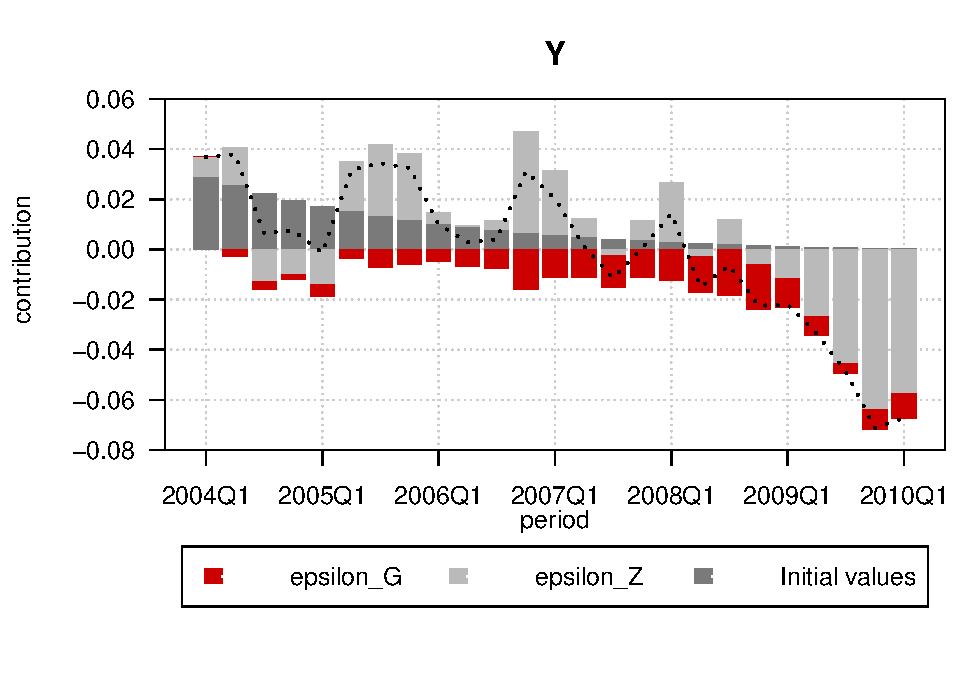
\includegraphics{figure/minimal-dsge6-1} 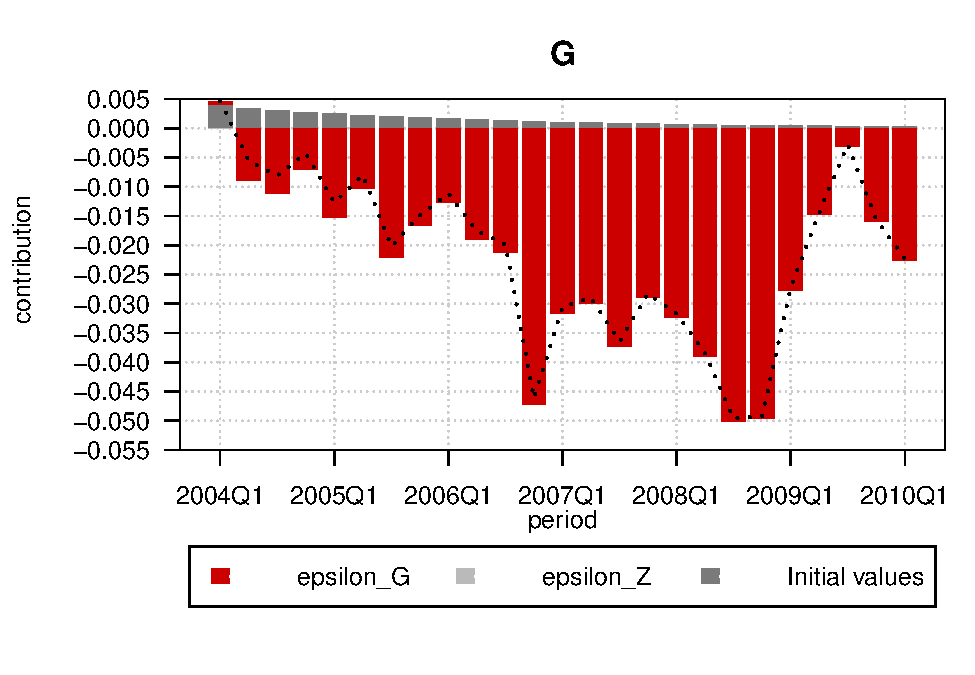
\includegraphics{figure/minimal-dsge6-2} \end{center}

\begin{Shaded}
\begin{Highlighting}[]
\CommentTok{# ###################################################################}
\CommentTok{# 6. forecast using the model}
\CommentTok{# forecast using point estimates of parameters}
\NormalTok{fc_res <-}\StringTok{ }\KeywordTok{forecast}\NormalTok{(}\DataTypeTok{model =}\NormalTok{ estimated_dsge_model,}
                   \DataTypeTok{data_set =}\NormalTok{ estimation_data,}
                   \DataTypeTok{observables =}\NormalTok{ observables,}
                   \DataTypeTok{variables =} \KeywordTok{c}\NormalTok{(}\StringTok{"Y"}\NormalTok{, }\StringTok{"G"}\NormalTok{),}
                   \DataTypeTok{horizon =} \DecValTok{20}\NormalTok{)}

\CommentTok{# forecast using posterior distribution}
\NormalTok{fc_res_post <-}\StringTok{ }\KeywordTok{forecast_posterior}\NormalTok{(}\DataTypeTok{est_results =}\NormalTok{ estimation_result,}
                                  \DataTypeTok{data_set =}\NormalTok{ estimation_data,}
                                  \DataTypeTok{observables =}\NormalTok{ observables,}
                                  \DataTypeTok{variables =} \KeywordTok{c}\NormalTok{(}\StringTok{"Y"}\NormalTok{, }\StringTok{"G"}\NormalTok{),}
                                  \DataTypeTok{horizon =} \DecValTok{20}\NormalTok{)}
\end{Highlighting}
\end{Shaded}

\begin{verbatim}
## The 250 parameter samples will be drawn from the posterior distribution 
##  
## 50 parameter samples (20 percent) have been already drawn from the posterior.
## 100 parameter samples (40 percent) have been already drawn from the posterior.
## 150 parameter samples (60 percent) have been already drawn from the posterior.
## 200 parameter samples (80 percent) have been already drawn from the posterior.
## 250 parameter samples (100 percent) have been already drawn from the posterior.
\end{verbatim}

\begin{Shaded}
\begin{Highlighting}[]
\CommentTok{#"The forecast_posterior function allows to create forecasts by sampling parameter values from the posterior distribution, solving model, and simulating it for the n-periods ahead. The initial values of state variables for the forecast are obtained by the application of Kalman smoother."}

\CommentTok{# plot forecasts}
\KeywordTok{plot_forecast}\NormalTok{(fc_res_post)}
\KeywordTok{plot_forecast}\NormalTok{(fc_res)}
\end{Highlighting}
\end{Shaded}

\begin{center}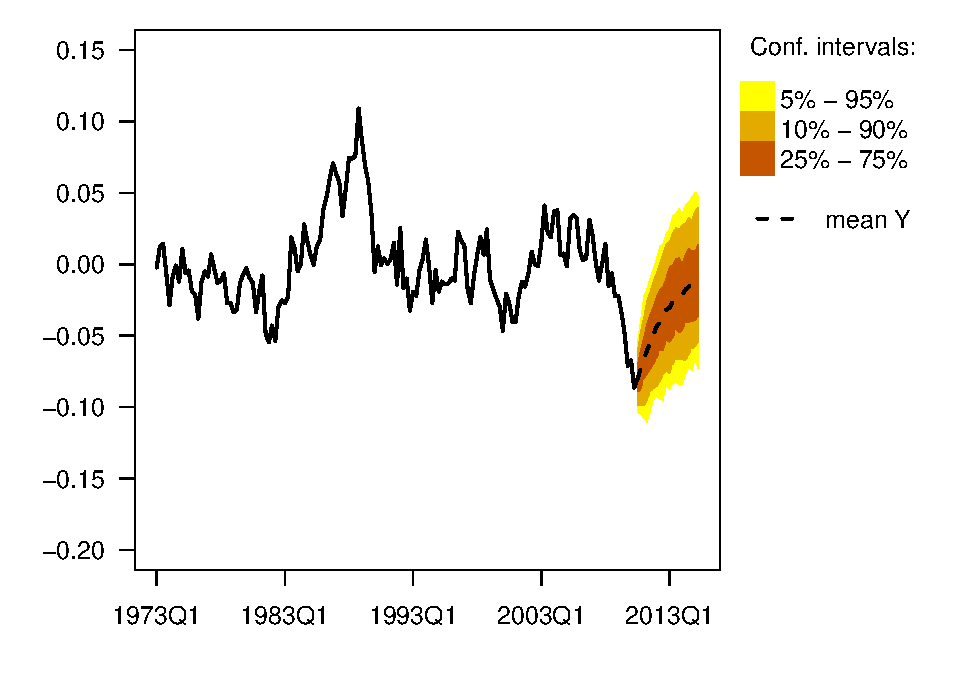
\includegraphics{figure/minimal-dsge7-1} 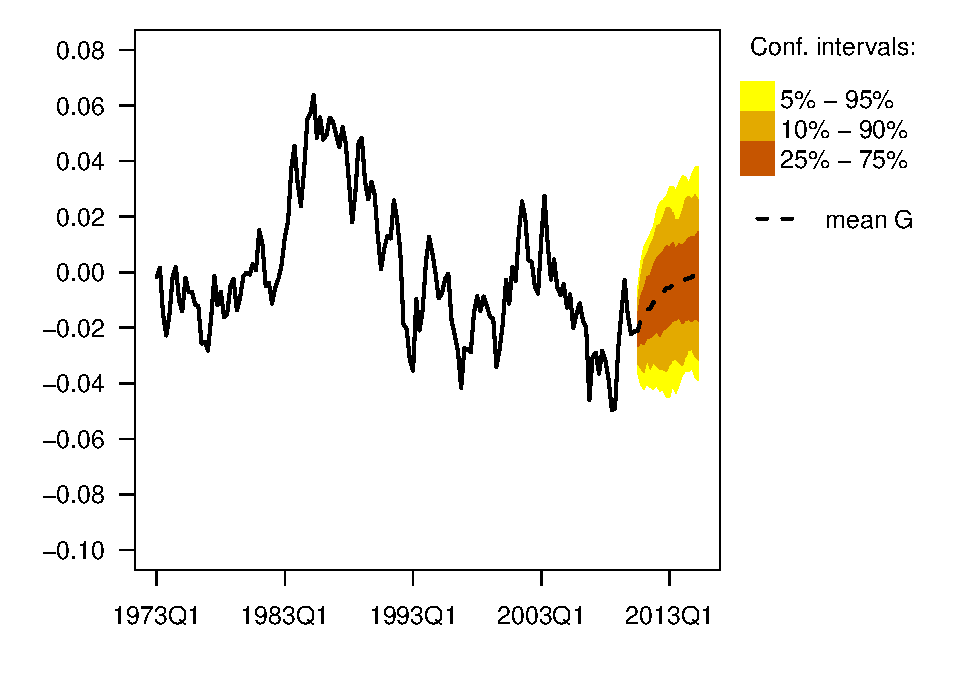
\includegraphics{figure/minimal-dsge7-2} 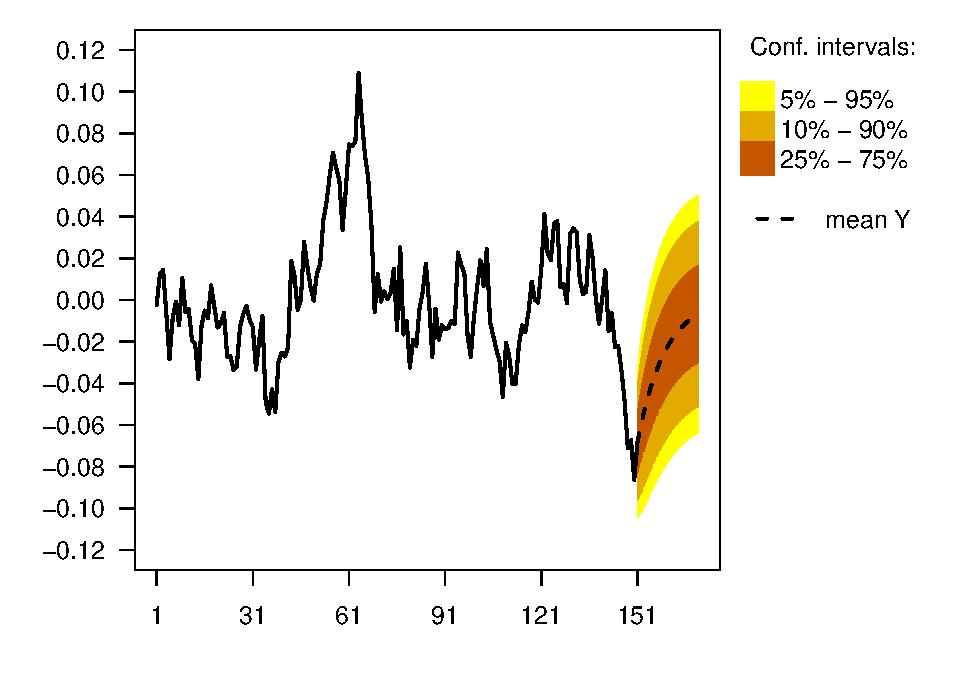
\includegraphics{figure/minimal-dsge7-3} 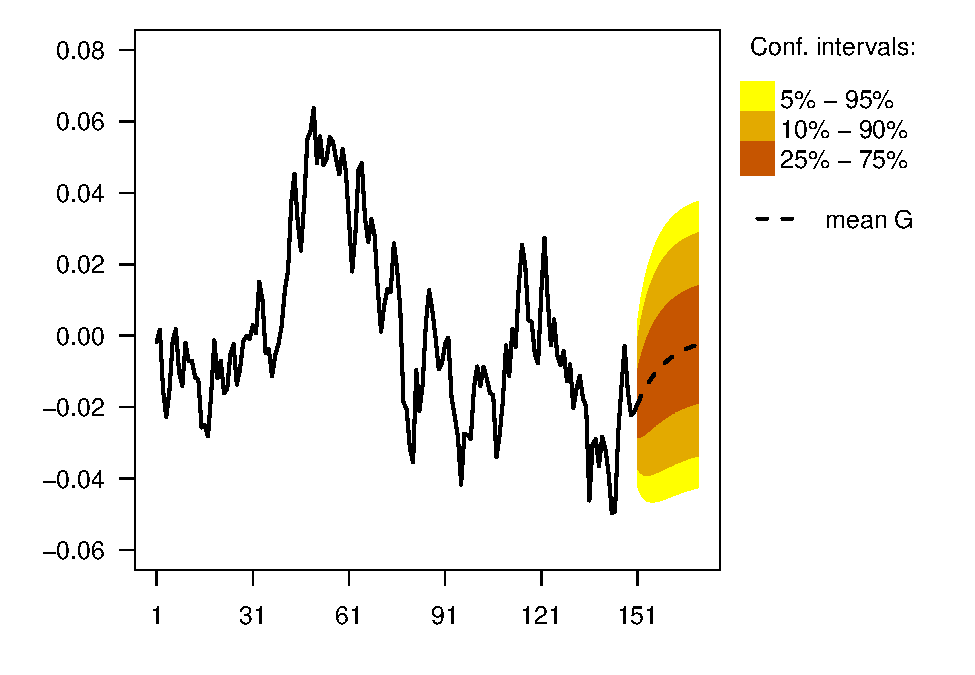
\includegraphics{figure/minimal-dsge7-4} \end{center}

% More bibliography
\bibliography{references.bib}

\end{document}
